% Use only LaTeX2e, calling the article.cls class and 12-point type.

\documentclass[12pt]{article}

\usepackage{polski}
\usepackage[utf8]{inputenc}


% Users of the {thebibliography} environment or BibTeX should use the
% scicite.sty package, downloadable from *Science* at
% www.sciencemag.org/about/authors/prep/TeX_help/ .
% This package should properly format in-text
% reference calls and reference-list numbers.

\usepackage{scicite}

% Use times if you have the font installed; otherwise, comment out the
% following line.

\usepackage{times}
\usepackage{amsmath}
\usepackage{graphicx}
\usepackage{algpseudocode}
\usepackage{amsmath}
\usepackage{algpseudocode}

% The preamble here sets up a lot of new/revised commands and
% environments.  It's annoying, but please do *not* try to strip these
% out into a separate .sty file (which could lead to the loss of some
% information when we convert the file to other formats).  Instead, keep
% them in the preamble of your main LaTeX source file.


% The following parameters seem to provide a reasonable page setup.

\topmargin 0.0cm
\oddsidemargin 0.2cm
\textwidth 16cm 
\textheight 21cm
\footskip 1.0cm


%The next command sets up an environment for the abstract to your paper.

\newenvironment{sciabstract}{%
\begin{quote} \bf}
{\end{quote}}


% If your reference list includes text notes as well as references,
% include the following line; otherwise, comment it out.

\renewcommand\refname{References and Notes}

% The following lines set up an environment for the last note in the
% reference list, which commonly includes acknowledgments of funding,
% help, etc.  It's intended for users of BibTeX or the {thebibliography}
% environment.  Users who are hand-coding their references at the end
% using a list environment such as {enumerate} can simply add another
% item at the end, and it will be numbered automatically.

\newcounter{lastnote}
\newenvironment{scilastnote}{%
\setcounter{lastnote}{\value{enumiv}}%
\addtocounter{lastnote}{+1}%
\begin{list}%
{\arabic{lastnote}.}
{\setlength{\leftmargin}{.22in}}
{\setlength{\labelsep}{.5em}}}
{\end{list}}


% Include your paper's title here

\title{Użycie hybrydowego Algorytmu Genetycznego z Symulowanym Wyżarzaniem w celu znajdowania minimalnych drzew rozpinających w wariancie kwadratowym} 


% Place the author information here.  Please hand-code the contact
% information and notecalls; do *not* use \footnote commands.  Let the
% author contact information appear immediately below the author names
% as shown.  We would also prefer that you don't change the type-size
% settings shown here.

\author
{Michał Drzał\\Marcin Paśko\\
\\
\normalsize{Akademia Górniczo-Hutnicza im. Adama Mickiewicza w Krakowie}\\
\normalsize{Wydział Informatyki Elektroniki i Telekomunikacji}\\
}

% Include the date command, but leave its argument blank.

\date{}



%%%%%%%%%%%%%%%%% END OF PREAMBLE %%%%%%%%%%%%%%%%



\begin{document} 

% Double-space the manuscript.

\baselineskip24pt

% Make the title.

\maketitle 



% Place your abstract within the special {sciabstract} environment.

\begin{sciabstract}
  Niniejszy dokument stanowi raport z wynikami projektu, relalizowanego z przedmiotu Stochastyczne Algorytmy Obliczeniowe, prowadzonego przed prof. dr hab. inż. Roberta Shaefera.
\end{sciabstract}



% In setting up this template for *Science* papers, we've used both
% the \section* command and the \paragraph* command for topical
% divisions.  Which you use will of course depend on the type of paper
% you're writing.  Review Articles tend to have displayed headings, for
% which \section* is more appropriate; Research Articles, when they have
% formal topical divisions at all, tend to signal them with bold text
% that runs into the paragraph, for which \paragraph* is the right
% choice.  Either way, use the asterisk (*) modifier, as shown, to
% suppress numbering.

\section*{Sformułowanie problemu}





Niech $G =(V,E)$ będzie nieskierowanym grafem ze zbiorem wierzchołków V i zbiorem krawędzi E. Problem kwadratowego minimalnego drzewa rozpinającego (QMSTP, quadratic minimum spanning tree) w którym każda krawędź posiada przypisany koszt $e_{g}$ oraz każda para krawędzi posiada koszt $c_{eg}$ i minimalizowany koszt drzewa rozpinającego $T= (V, E(T))$ jest wyrazony:
$$ F(T) = \sum_{e \in E(T) } c_e + \sum_{(e,g) \in \Psi (T)} c_{eg} $$

 $\Psi (T)$ oznacza zbiór wszystkich par krawędzi znajdujących sie w drzewie $T$. Rozwiązania QMSTP znajdują zastosowanie w telekomunikacji, logistyce i dystrybucji energii.
 
 Problem QMST jest NP-trudny \cite{Assad}, przez co optymalny algorytm rozwiązujący go w czasie wielomianowym istnieje tylko jesli $P=NP$. Uzasadnione jest wiec wykorzystanie do znalezienia rozwiązania jednej z wielu dostępnych metaheurystyk.
 
 \section{Wykorzystana metaheurystyka}

Zastosowanie reguł zaczerpniętych z procesów ewolucyjnych jest powszechnie stosowana praktyka podczas rozwiązywania problemów ewolucyjnych. Na potrzeby naszego projektu wykorzystaliśmy algorytm genetyczny jako matryce do stworzenia właściwego algorytmu. W trakcie rozwiązywania QMSTP utrzymujemy populacje rozwiązań, gdzie pojedynczy osobnik stanowi pojedyncze drzewo rozpinające w grafie $G$. Reprezentowany jest w postaci grafu odpowiadającego liście krawędzi z oryginalnego grafu. Korzystając z wzoru na koszt drzewa rozpinającego ustalana jest jakość rozwiązania. Następnie droga selekcji turniejowej wybierane są rozwiązania do krzyżowania. Rozwiązania powstałe wskutek krzyżowania zamieniają najsłabsze rozwiązania z populacji. Oprócz krzyżowania rozwiązania z pewnym prawdopodobieństwem poddawane są operacji losowej mutacji.


W celu ustalenia początkowej populacji konieczne jest wygenerowanie losowych grafów będących drzewami rozpinającymi (niekoniecznie minimalnymi). Ważne jest aby rozkład z którego losowane są drzewa rozpinające był rozkładem jednostajnym, dzięki czemu możliwe będzie przeszukiwanie przestrzeni rozwiązań bez uprzywilejowanego traktowania części rozwiązań. Losowe drzewo rozpinające uzyskuje się rozpoczynając błądzenie losowe zaczynając od losowego wierzchołka.

\begin{figure}[h!]
 \centering
\begin{algorithmic}
\Function{RandomTree}{}
\State $r\gets \Call{RandomVertex}{nil}$
\For{ $i < n$}
    \State $InTree[i] \gets false $
    \State $i\gets i+1$
\EndFor
\State $Next[r] \gets nil $
\State $InTree[r] \gets true $


\For{ $i < n$}
    \State $u \gets 1 $
    \While{not InTree[u]}
        \State $Next[u] \gets \Call{RandomSuccessor}{u}$
        \State $u \gets Next[u]$
    \EndWhile
    \State $u\gets i$
    \While{not InTree[u]}
        \State $InTree[u] \gets true$
        \State $u \gets Next[u]$
    \EndWhile
   
    \State $i\gets i+1$
\EndFor


\Return Next

\EndFunction

\end{algorithmic}
\caption{Algorytm generujący losowe drzewo rozpinające}
\end{figure}


Operator mutacji opiera się na usunięciu losowej krawędzi z mutowanego drzewa rozpinającego oraz połączeniu powstałych w ten sposób dwóch spójnych podgrafów inna krawędzią, wylosowywaną spośród wszystkich możliwych.


\begin{figure}[h!]
 \centering
\begin{algorithmic}
\Function{MutateTree}{}
\State $u\gets \Call{RandomVertex}{nil}$
\State $v\gets \Call{NeighbourVertices}{u}$
\State $\Call{RemoveEdge}{u,v}$

\State $u_{vertices}\gets \Call{AccessibleVertices}{u}$
\State $v_{vertices}\gets \Call{AccessibleVertices}{v}$
\State $edges \gets \Call{PossibleEdges}{u_{vertices}, v_{vertices}}$
\State $edge \gets \Call{RandomSelect}{edges}$
\State $\Call{AddEdge}{edge[0],edge[1]}$

\EndFunction

\end{algorithmic}
\caption{Algorytm mutujący wybrane drzewo rozpinające}
\end{figure}
 
 
Operator krzyżowania na podstawie dwóch osobników tworzy nowe rozwiązanie posiadające cechy zarówno jednego jak i drugiego osobnika. w pierwotnej wersji operator krzyżowania opierał się na wybraniu największego, wspólnego, spójnego podgrafu i generacji reszty grafu błądzeniem losowym. W testach okazało się jednak, że tak zdefiniowany operator generuje zbyt losowe wyniki. Obecny operator sumuje ze sobą zbiory krawędzi rodziców i w tak powstałym grafie znajduje drzewo rozpinające.
 
 
 
\begin{figure}[h!]
 \centering
\begin{algorithmic}
\Function{Crossover}{parent1, parent2}
\State $graph \gets \Call{Compose}{parent1, parent2}$
\State $offspring \gets \Call{RandomSpanningTree}{graph}$
\Return $offspring$

\EndFunction

\end{algorithmic}
\caption{Algorytm dokonujacy operacji krzyzowania}
\end{figure}
 
 
W projekcie wykorzystano również mechanizmy zaczerpnięte z algorytmu symulowanego wyżarzania. Jest to algorytm wzorowany procesie wyżarzania stosowanego w metalurgii. Opiera się ono o stopniowym, kontrolowanym zmniejszaniu temperatury metalu celem optymalizacji (minimalizacji) energii swobodnej układu. Opierając się na tym mechanizmie, część parametrów procesu ewolucyjnego również podlega procesowi powolnej zmiany według ustalonego planu, należą do nich:

\begin{itemize}
  \item prawdopodobieństwo mutacji
  \item wielkość turnieju
\end{itemize}




 \section{Zbior testowy i wyniki}


 Do testów wykorzystano benchmark udostępniony przez Roberto Cordone\cite{Bechmark}. Zawiera on zbiór grafów różniących się od siebie:
 
 \begin{itemize}
  \item ilością wierzchołków (od 10 do 50 wierzchołków)
  \item gęstością grafu ($\frac{1}{3}, \frac{2}{3}, 1$)
  \item zakresem kosztów krawędzi i kosztów pomiędzy parami krawędzi (dwa dyskretne zakresy: 1-10,1-100)
\end{itemize}

Do testów zostały wybrane 3 grafy odpowiednio z: 10, 15 i 20 wierzchołkami. Wszystkie grafy są grafami pełnymi oraz wartości kosztów znajdują się w zakresie: 1-100. Dysponujemy dla nich również najlepszymi uzyskanymi rezultatami, odpowiednio: 2197, 5879 i 11101\cite{Results}.

\section*{Wyniki}

Niniejszy rozdział stanowi prezentację wyników. Wykonaliśmy łącznie 3 eksperymenty, każdy dla 3 rozmiarów danych. Wyniki w każdym przypadku zostały uśrednione dla 3 przebiegów. Na każdym wykresie przedstawiono wagę drzewa dla przeciętnego osobnika w populacji. Os X stanowi ilość ewaluacji funkcji celu.

Poniższe trzy wykresy stanowią przypadek porównawczy dla zwykłego algorytmu genetycznego z selekcją turniejową.

Mały rozmiar danych:

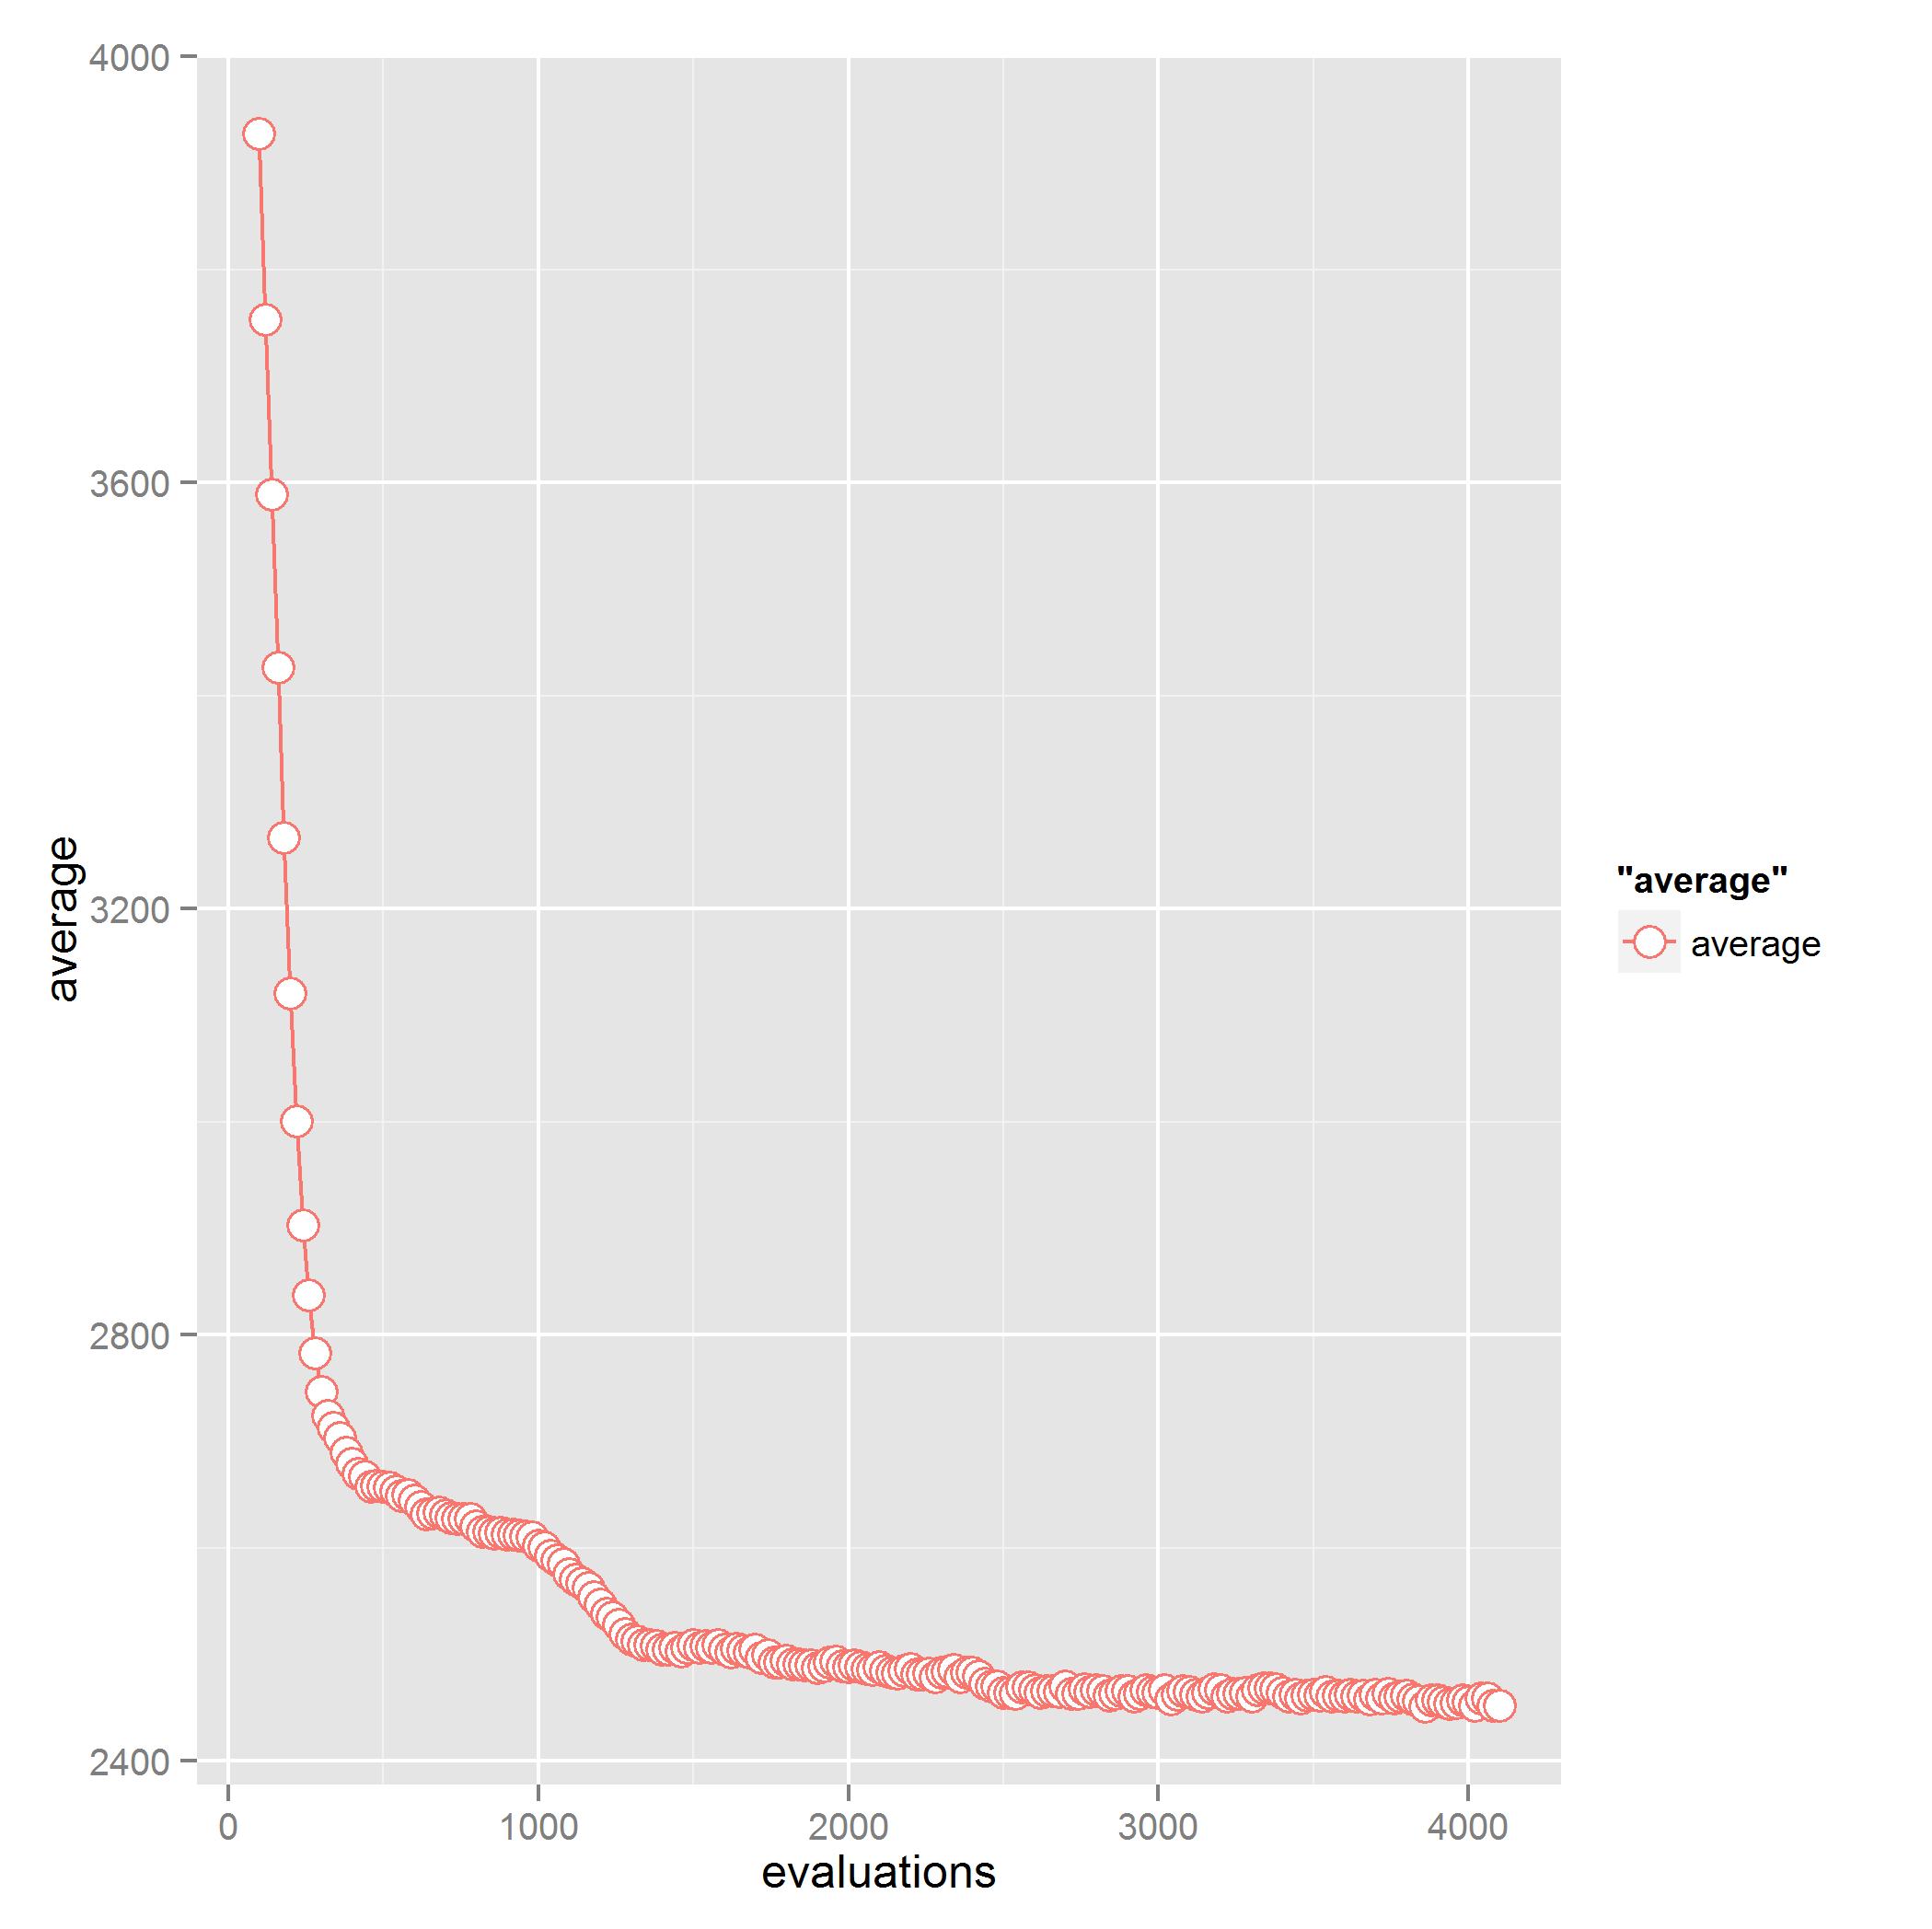
\includegraphics[]{simple_graph0.png}

Średni rozmiar danych:

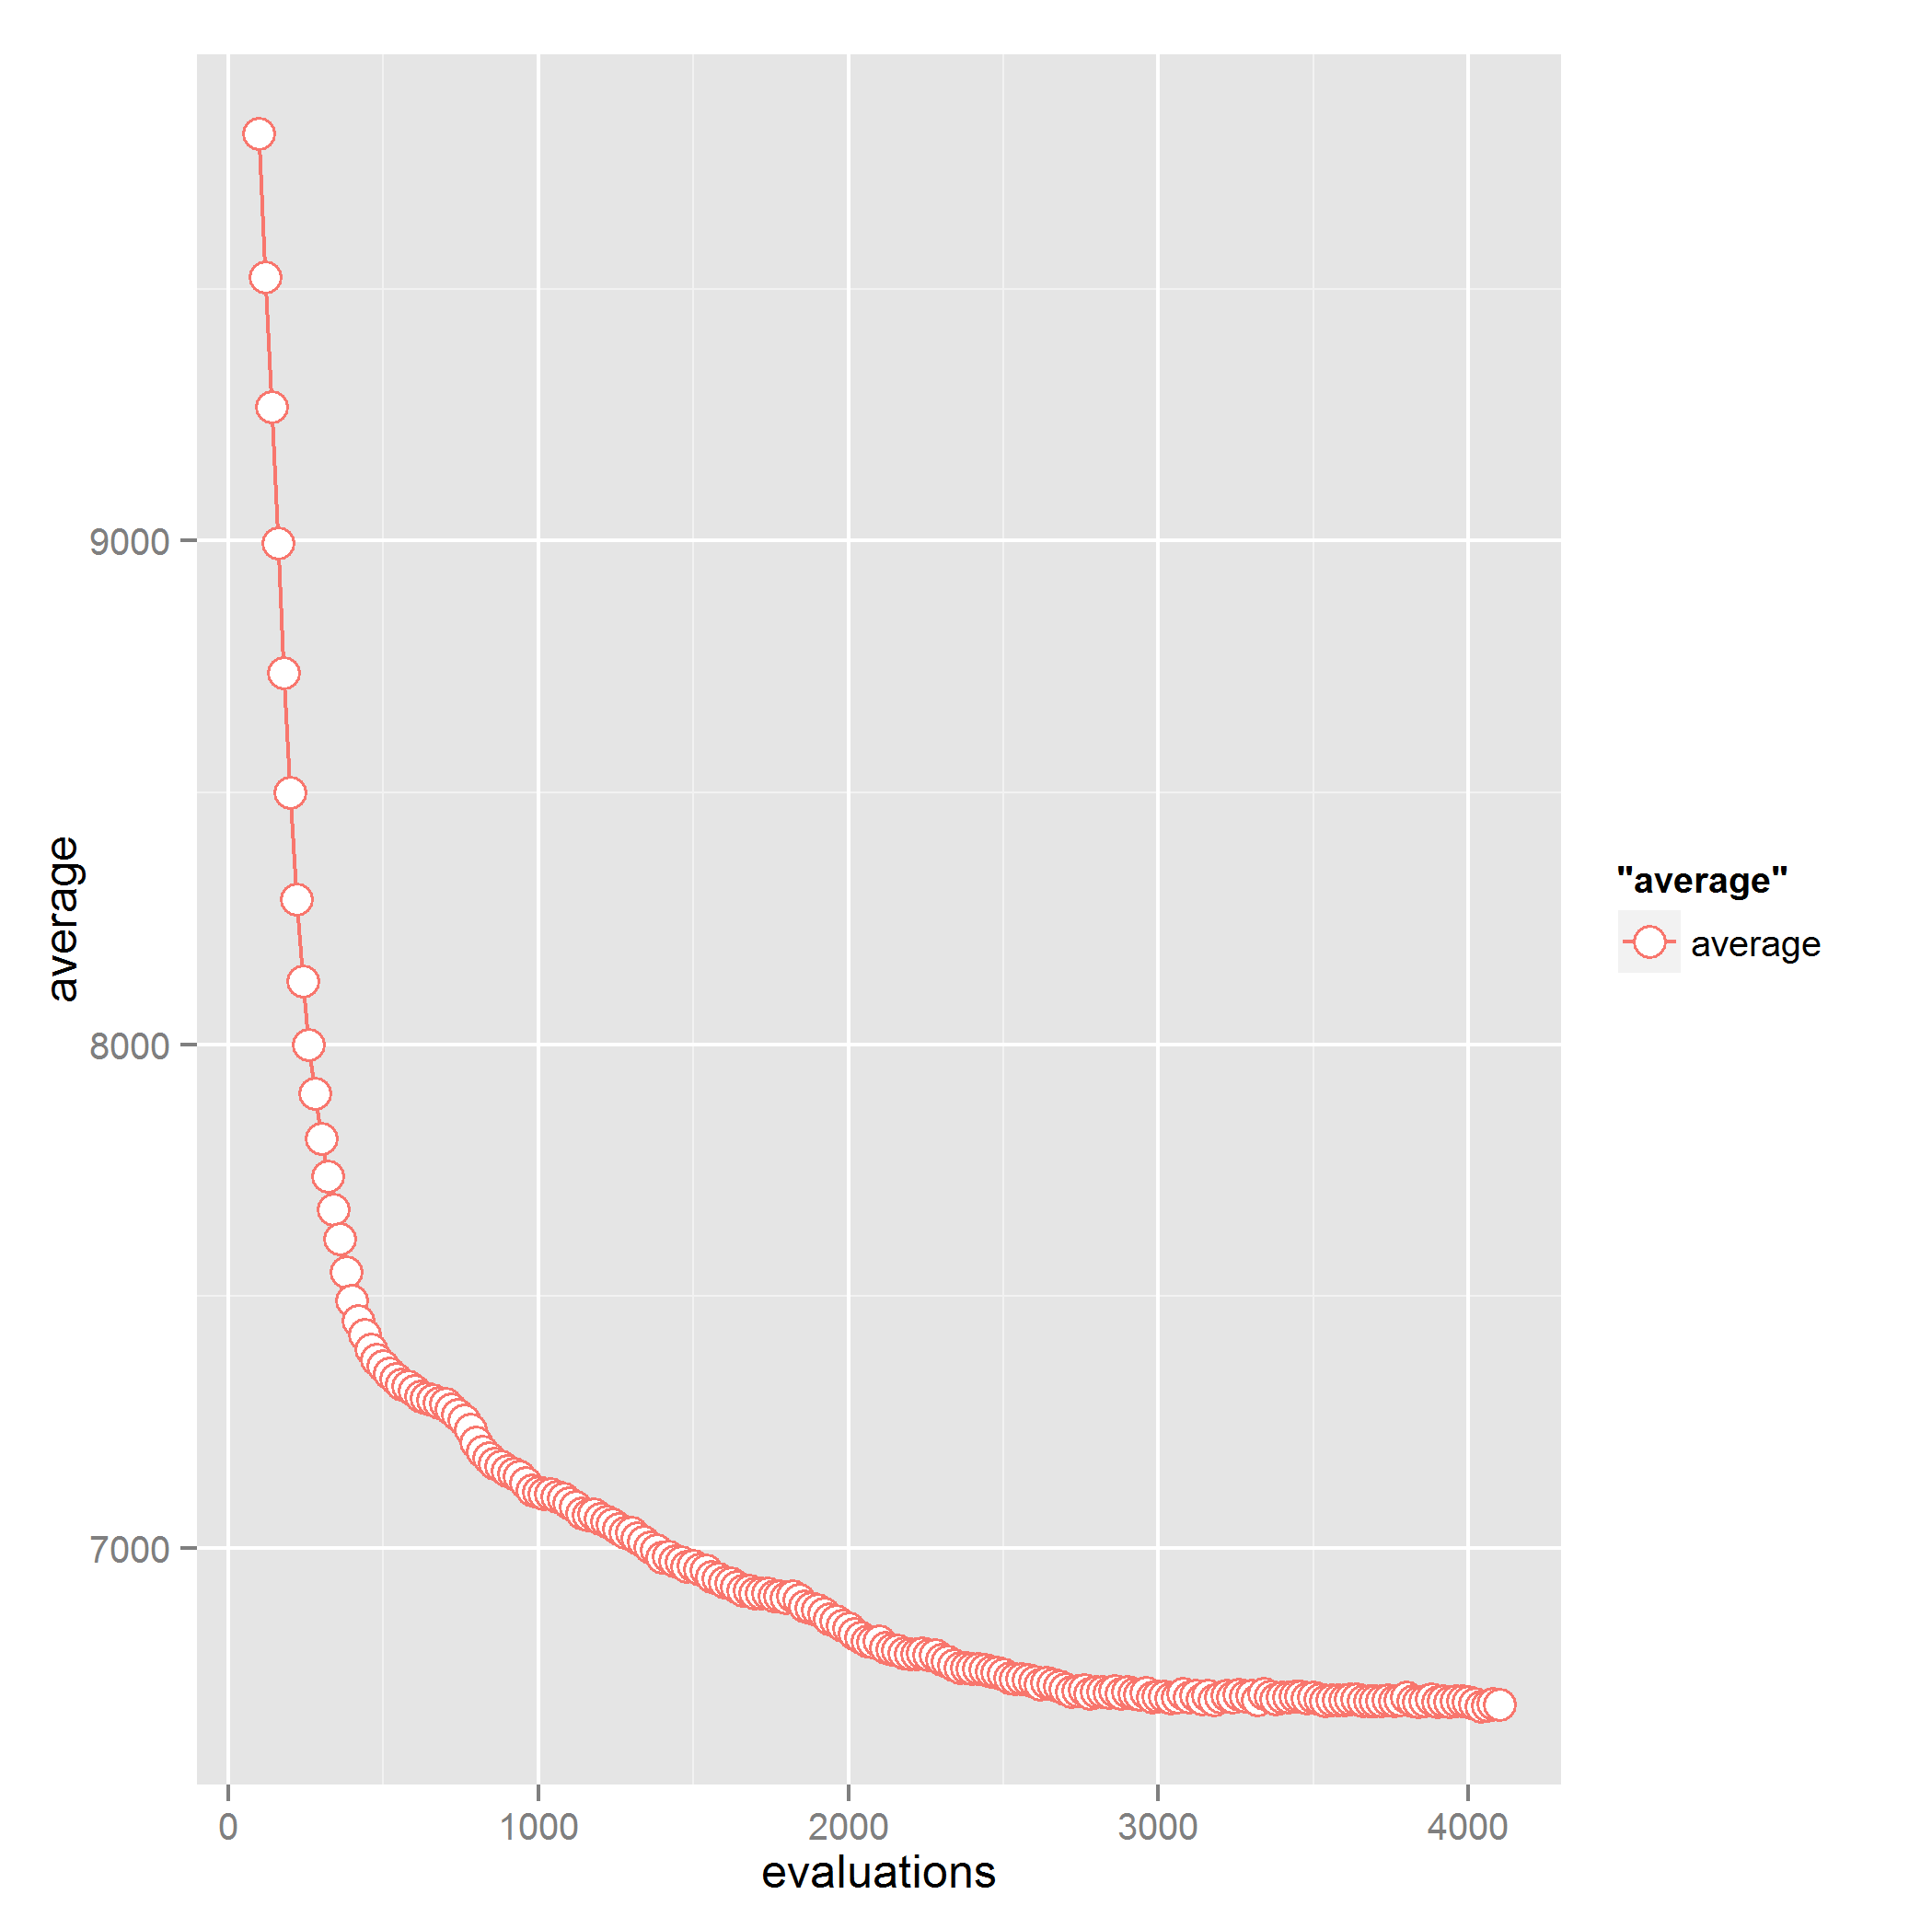
\includegraphics[]{simple_graph1.png}

Duży rozmiar danych:

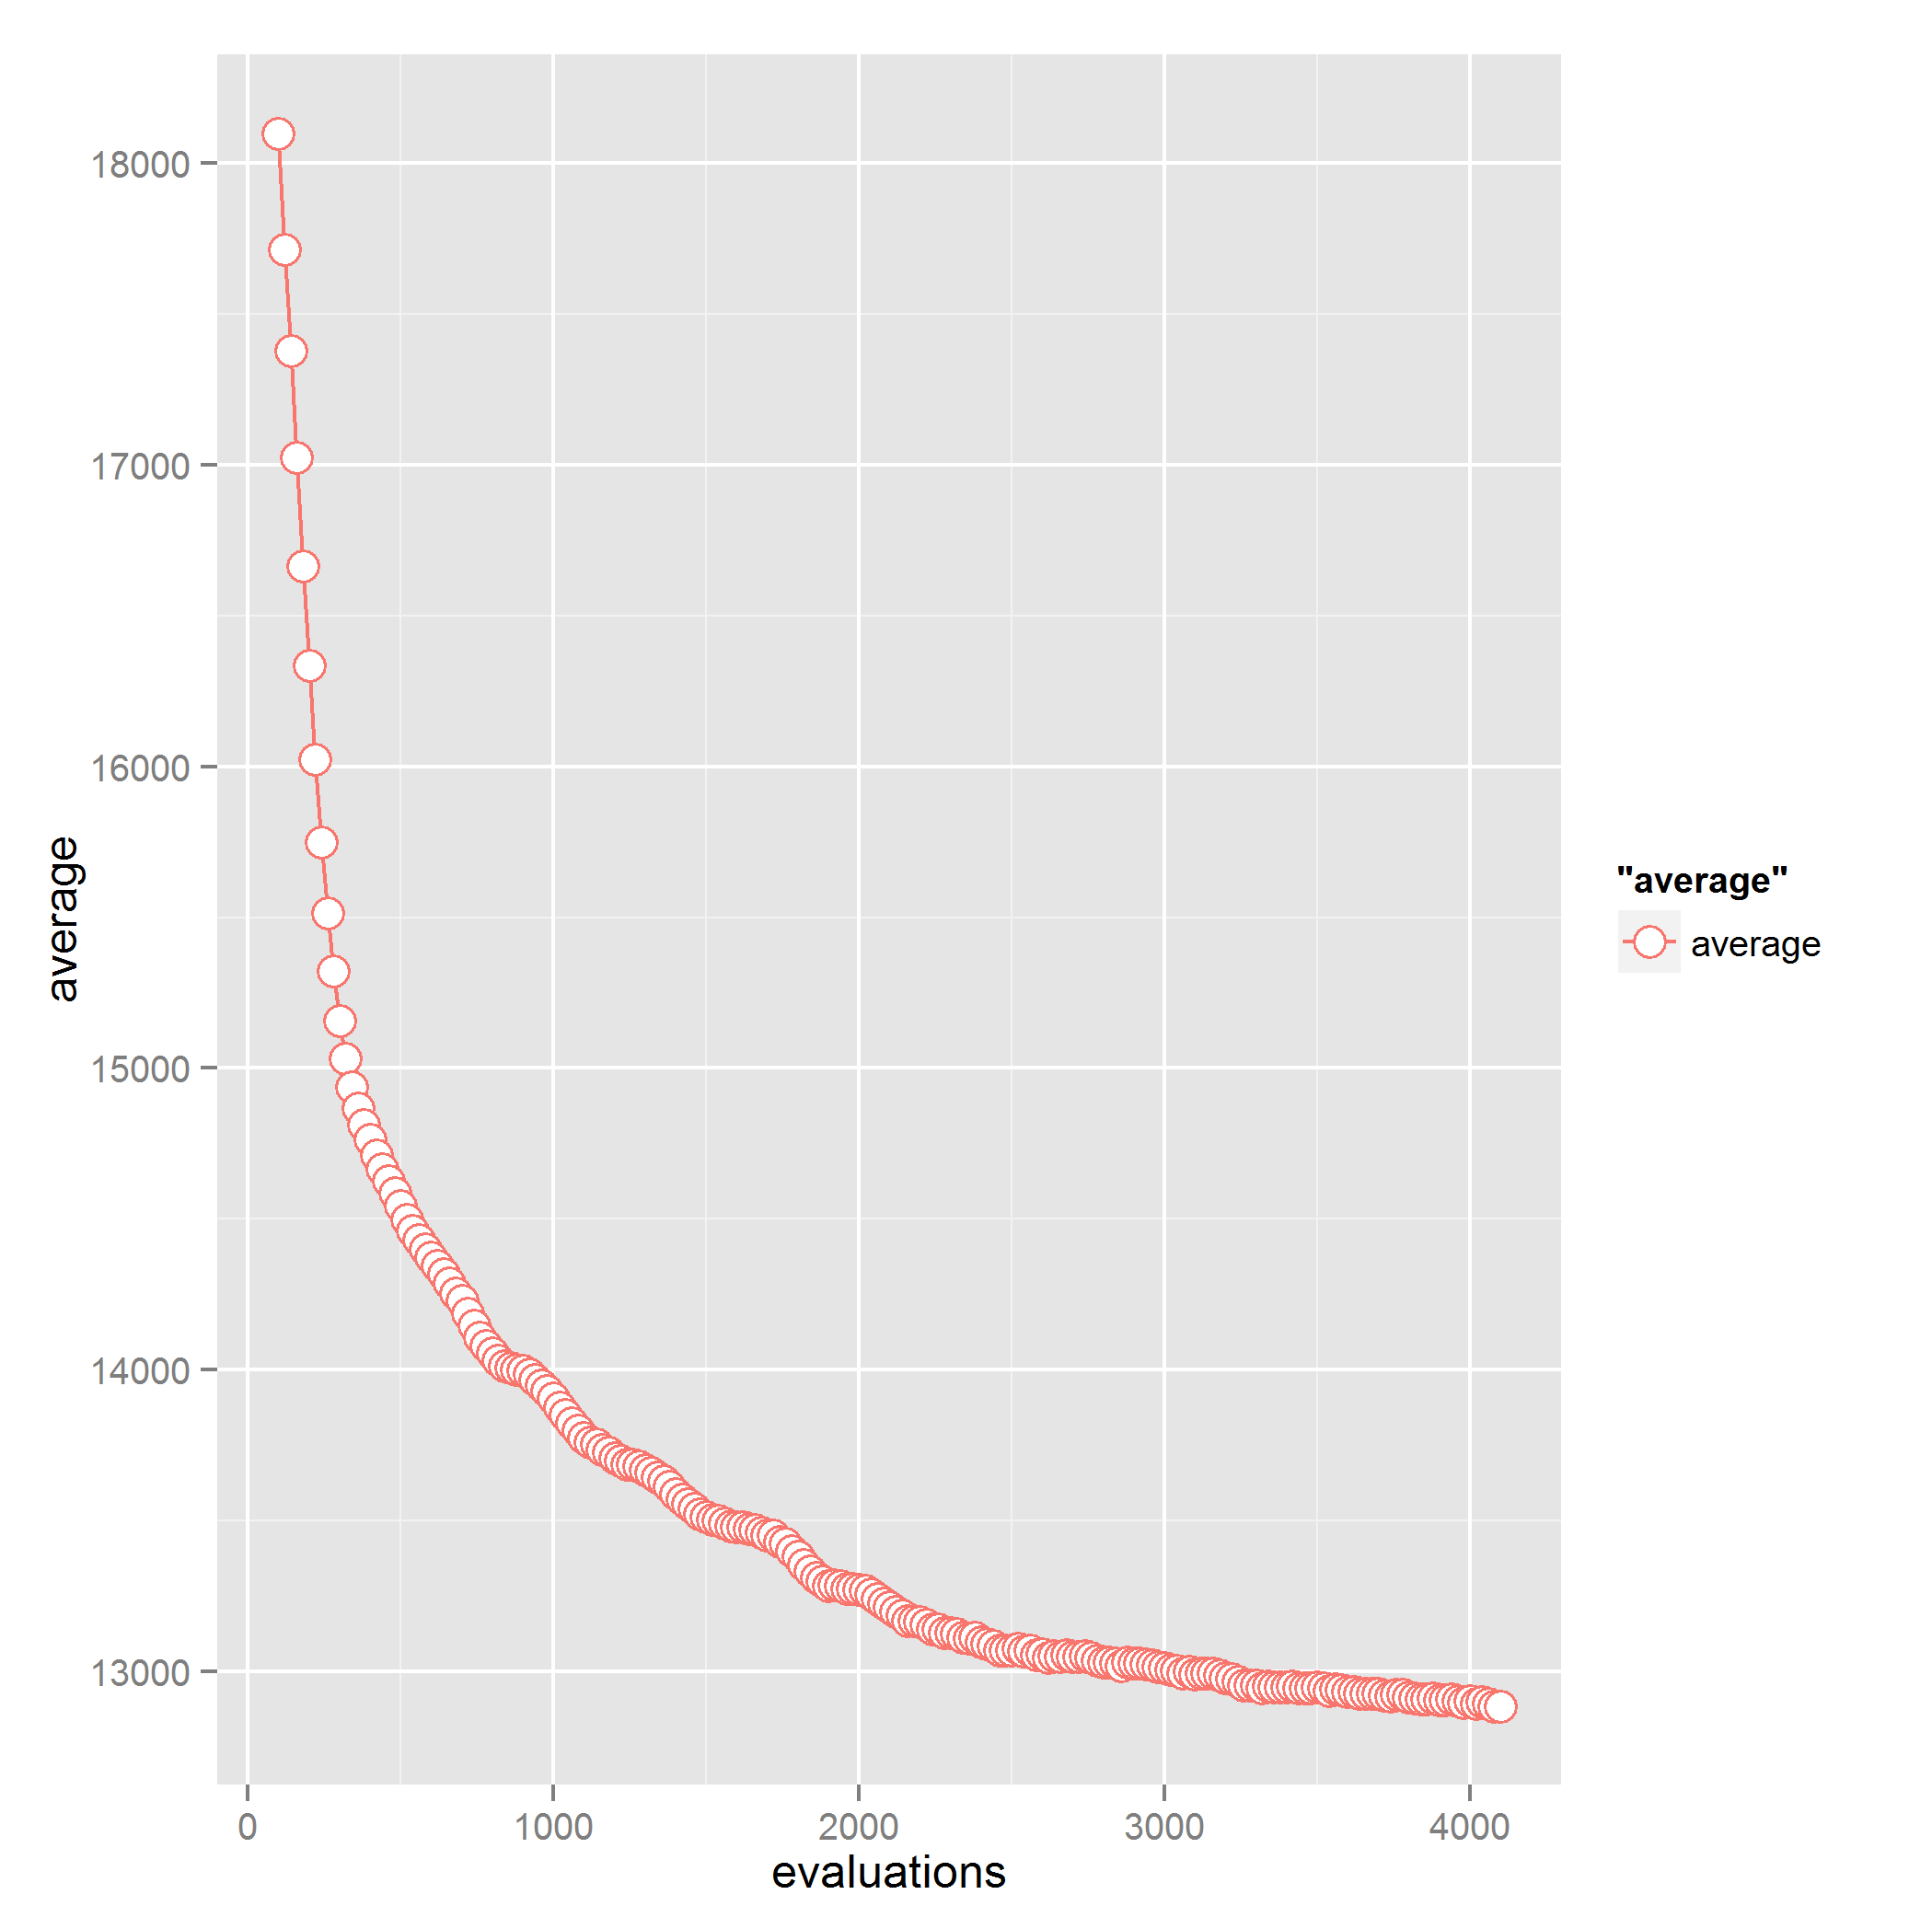
\includegraphics[]{simple_graph2.png}

Kolejne wyniki pochodzą z hybrydy algorytmu symulowanego wyżarzania, gdzie wychładzamy prawdopodobieństwo mutacji, które na początku miało dużą wartość np 1, a następnie jest wychładzane wykładniczo do bardzo małej wartości.

Mały rozmiar danych:

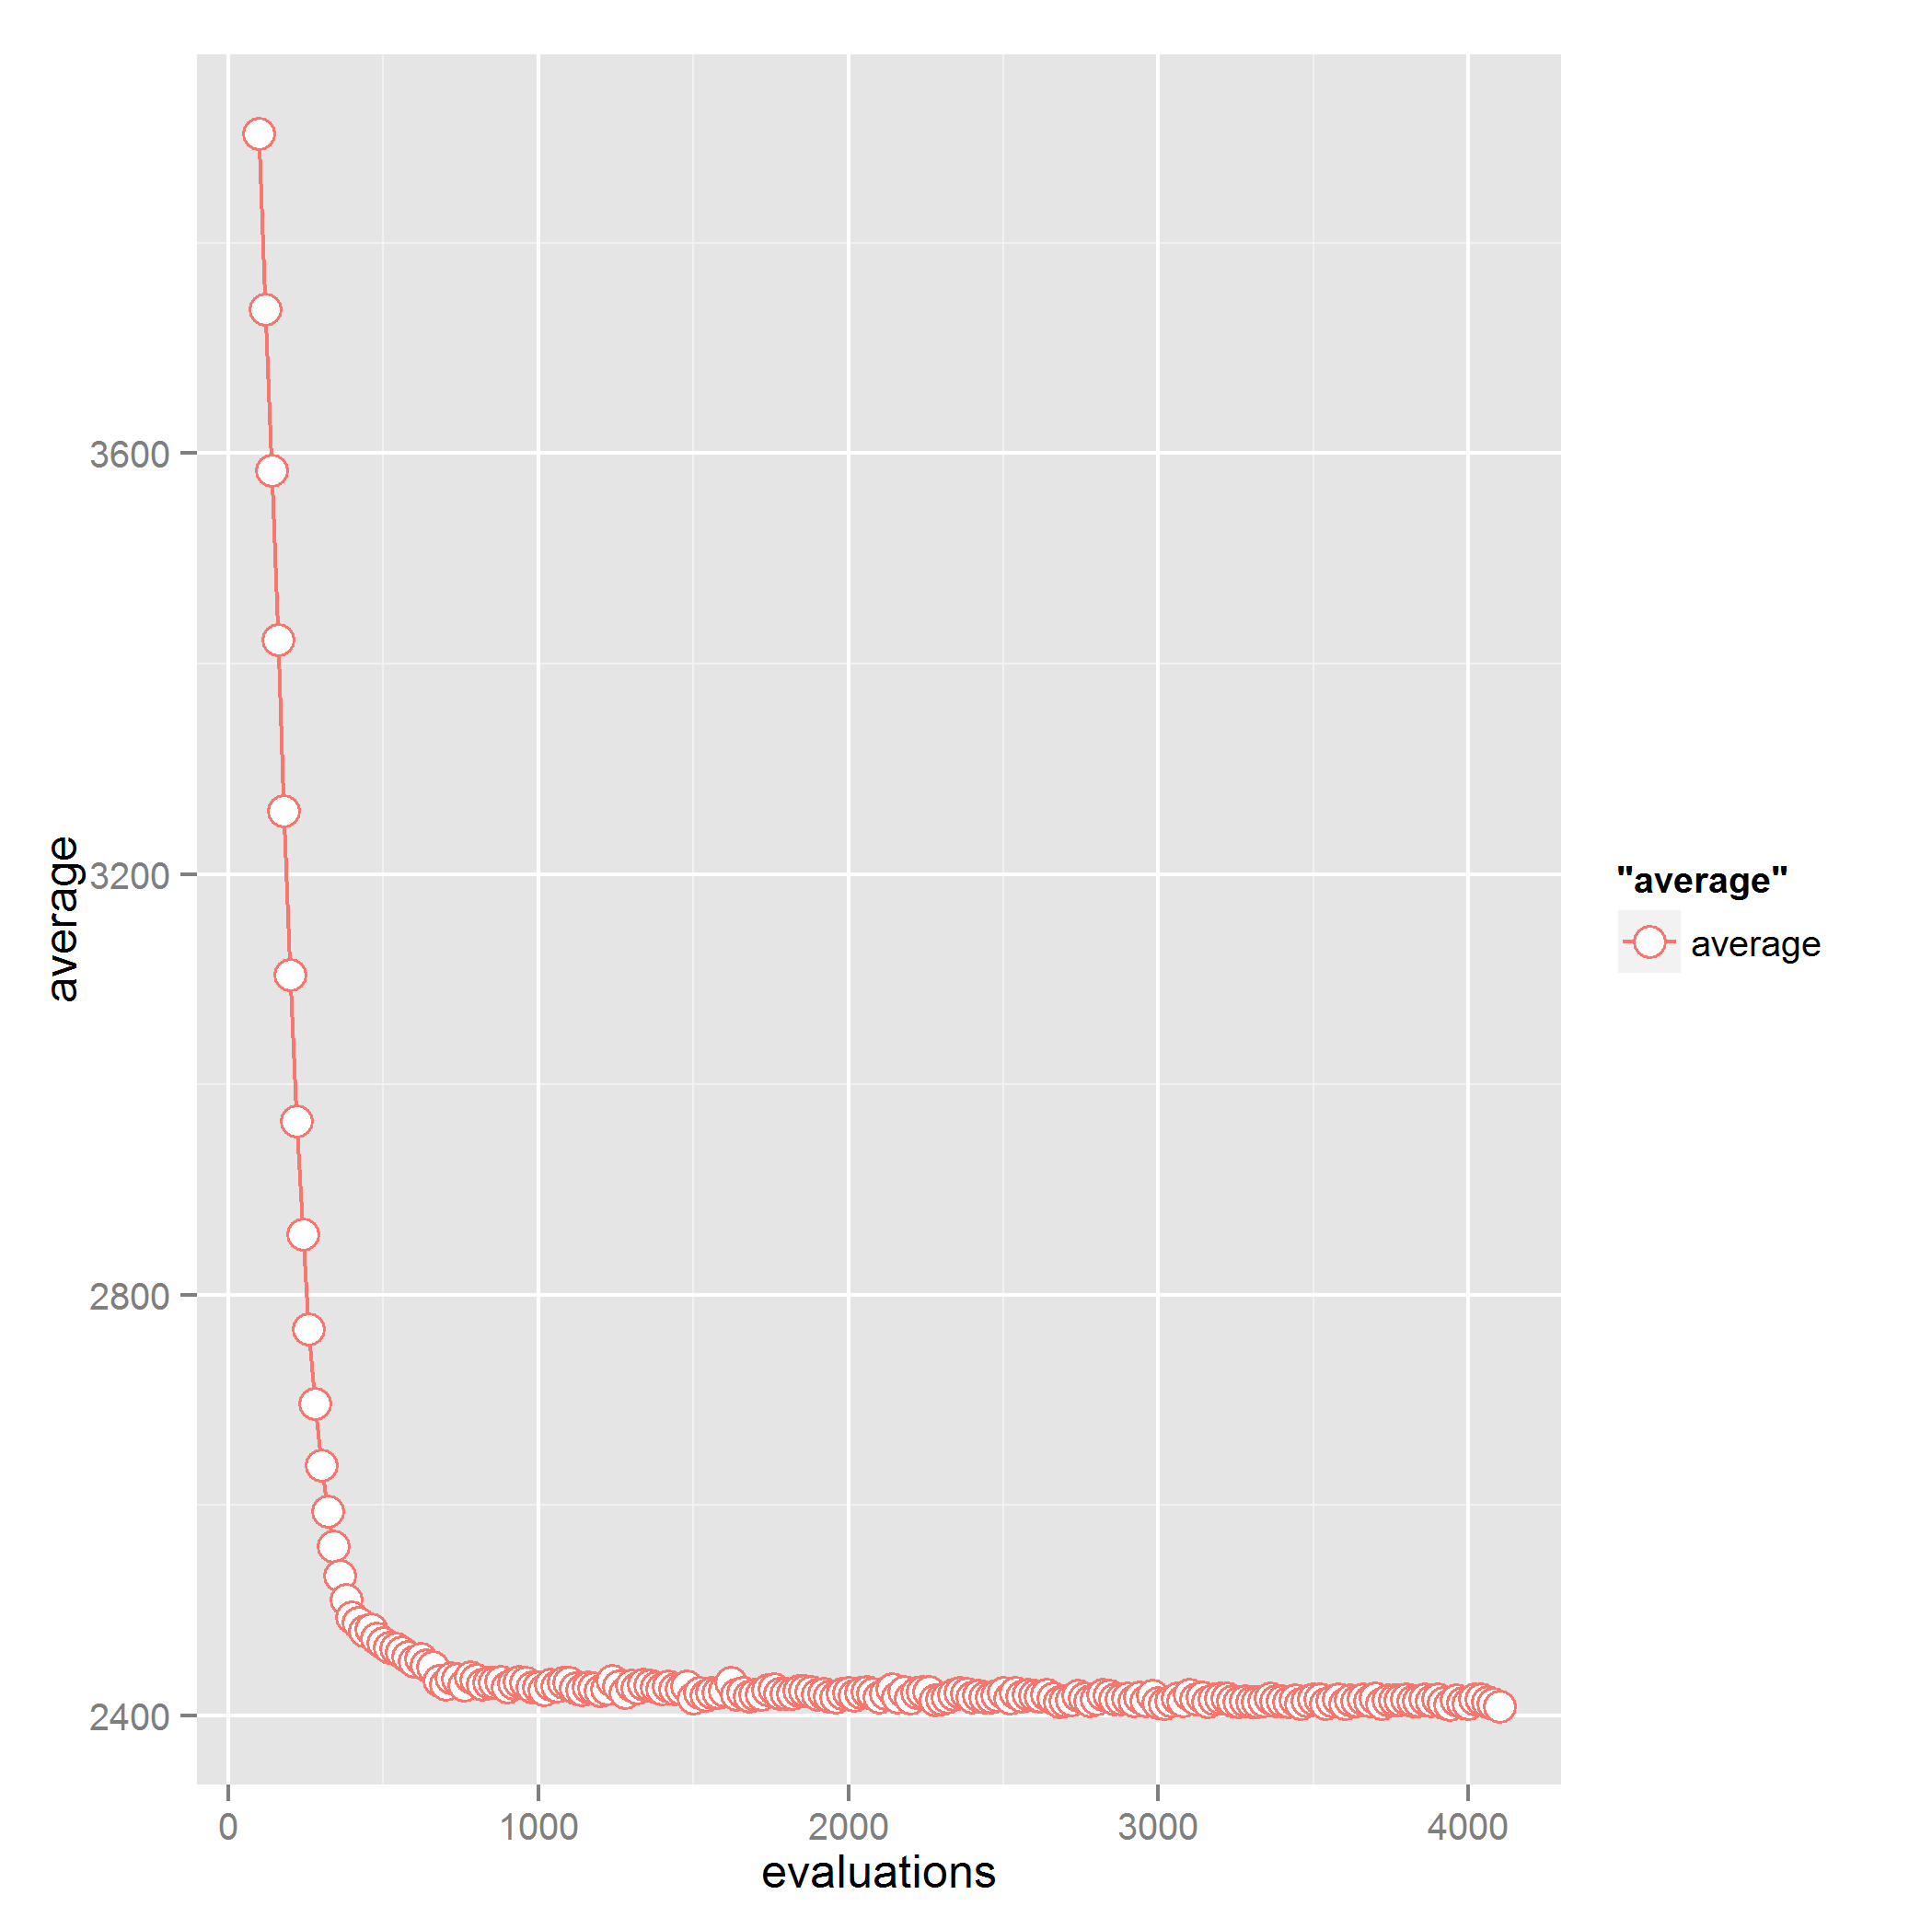
\includegraphics[]{mutation_cooling_graph0.png}

Średni rozmiar danych:

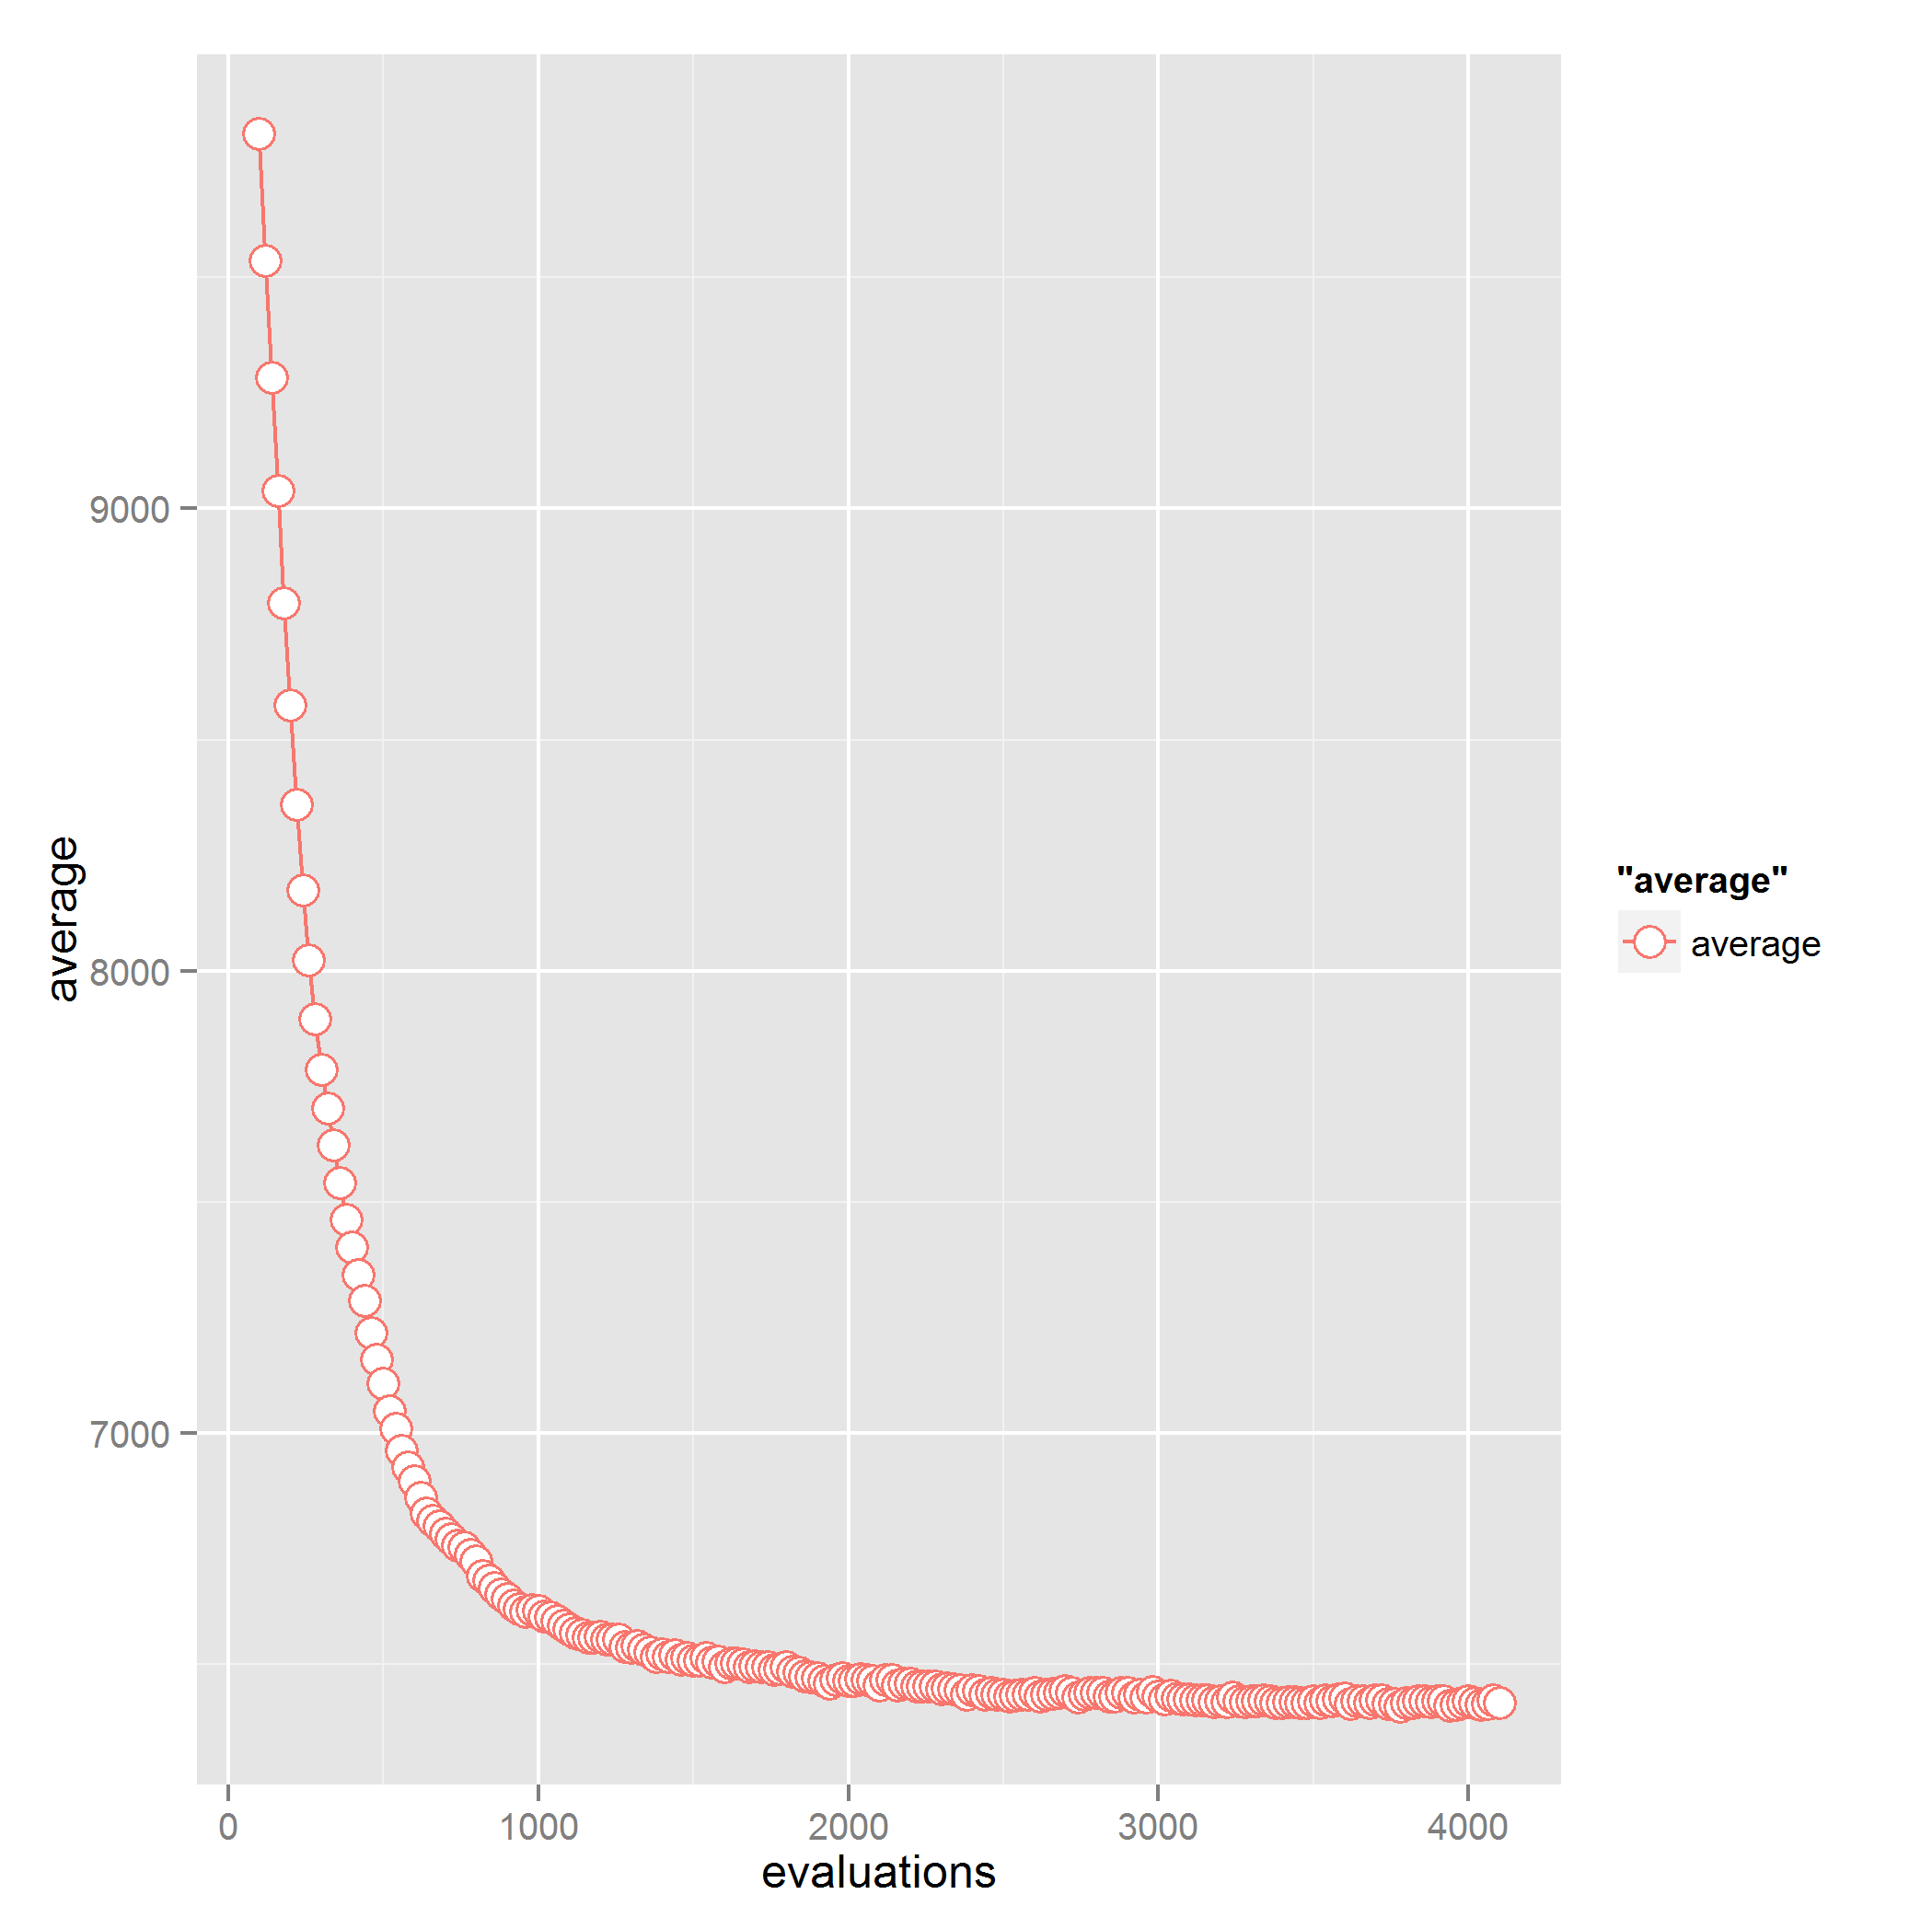
\includegraphics[]{mutation_cooling_graph1.png}

Duży rozmiar danych:

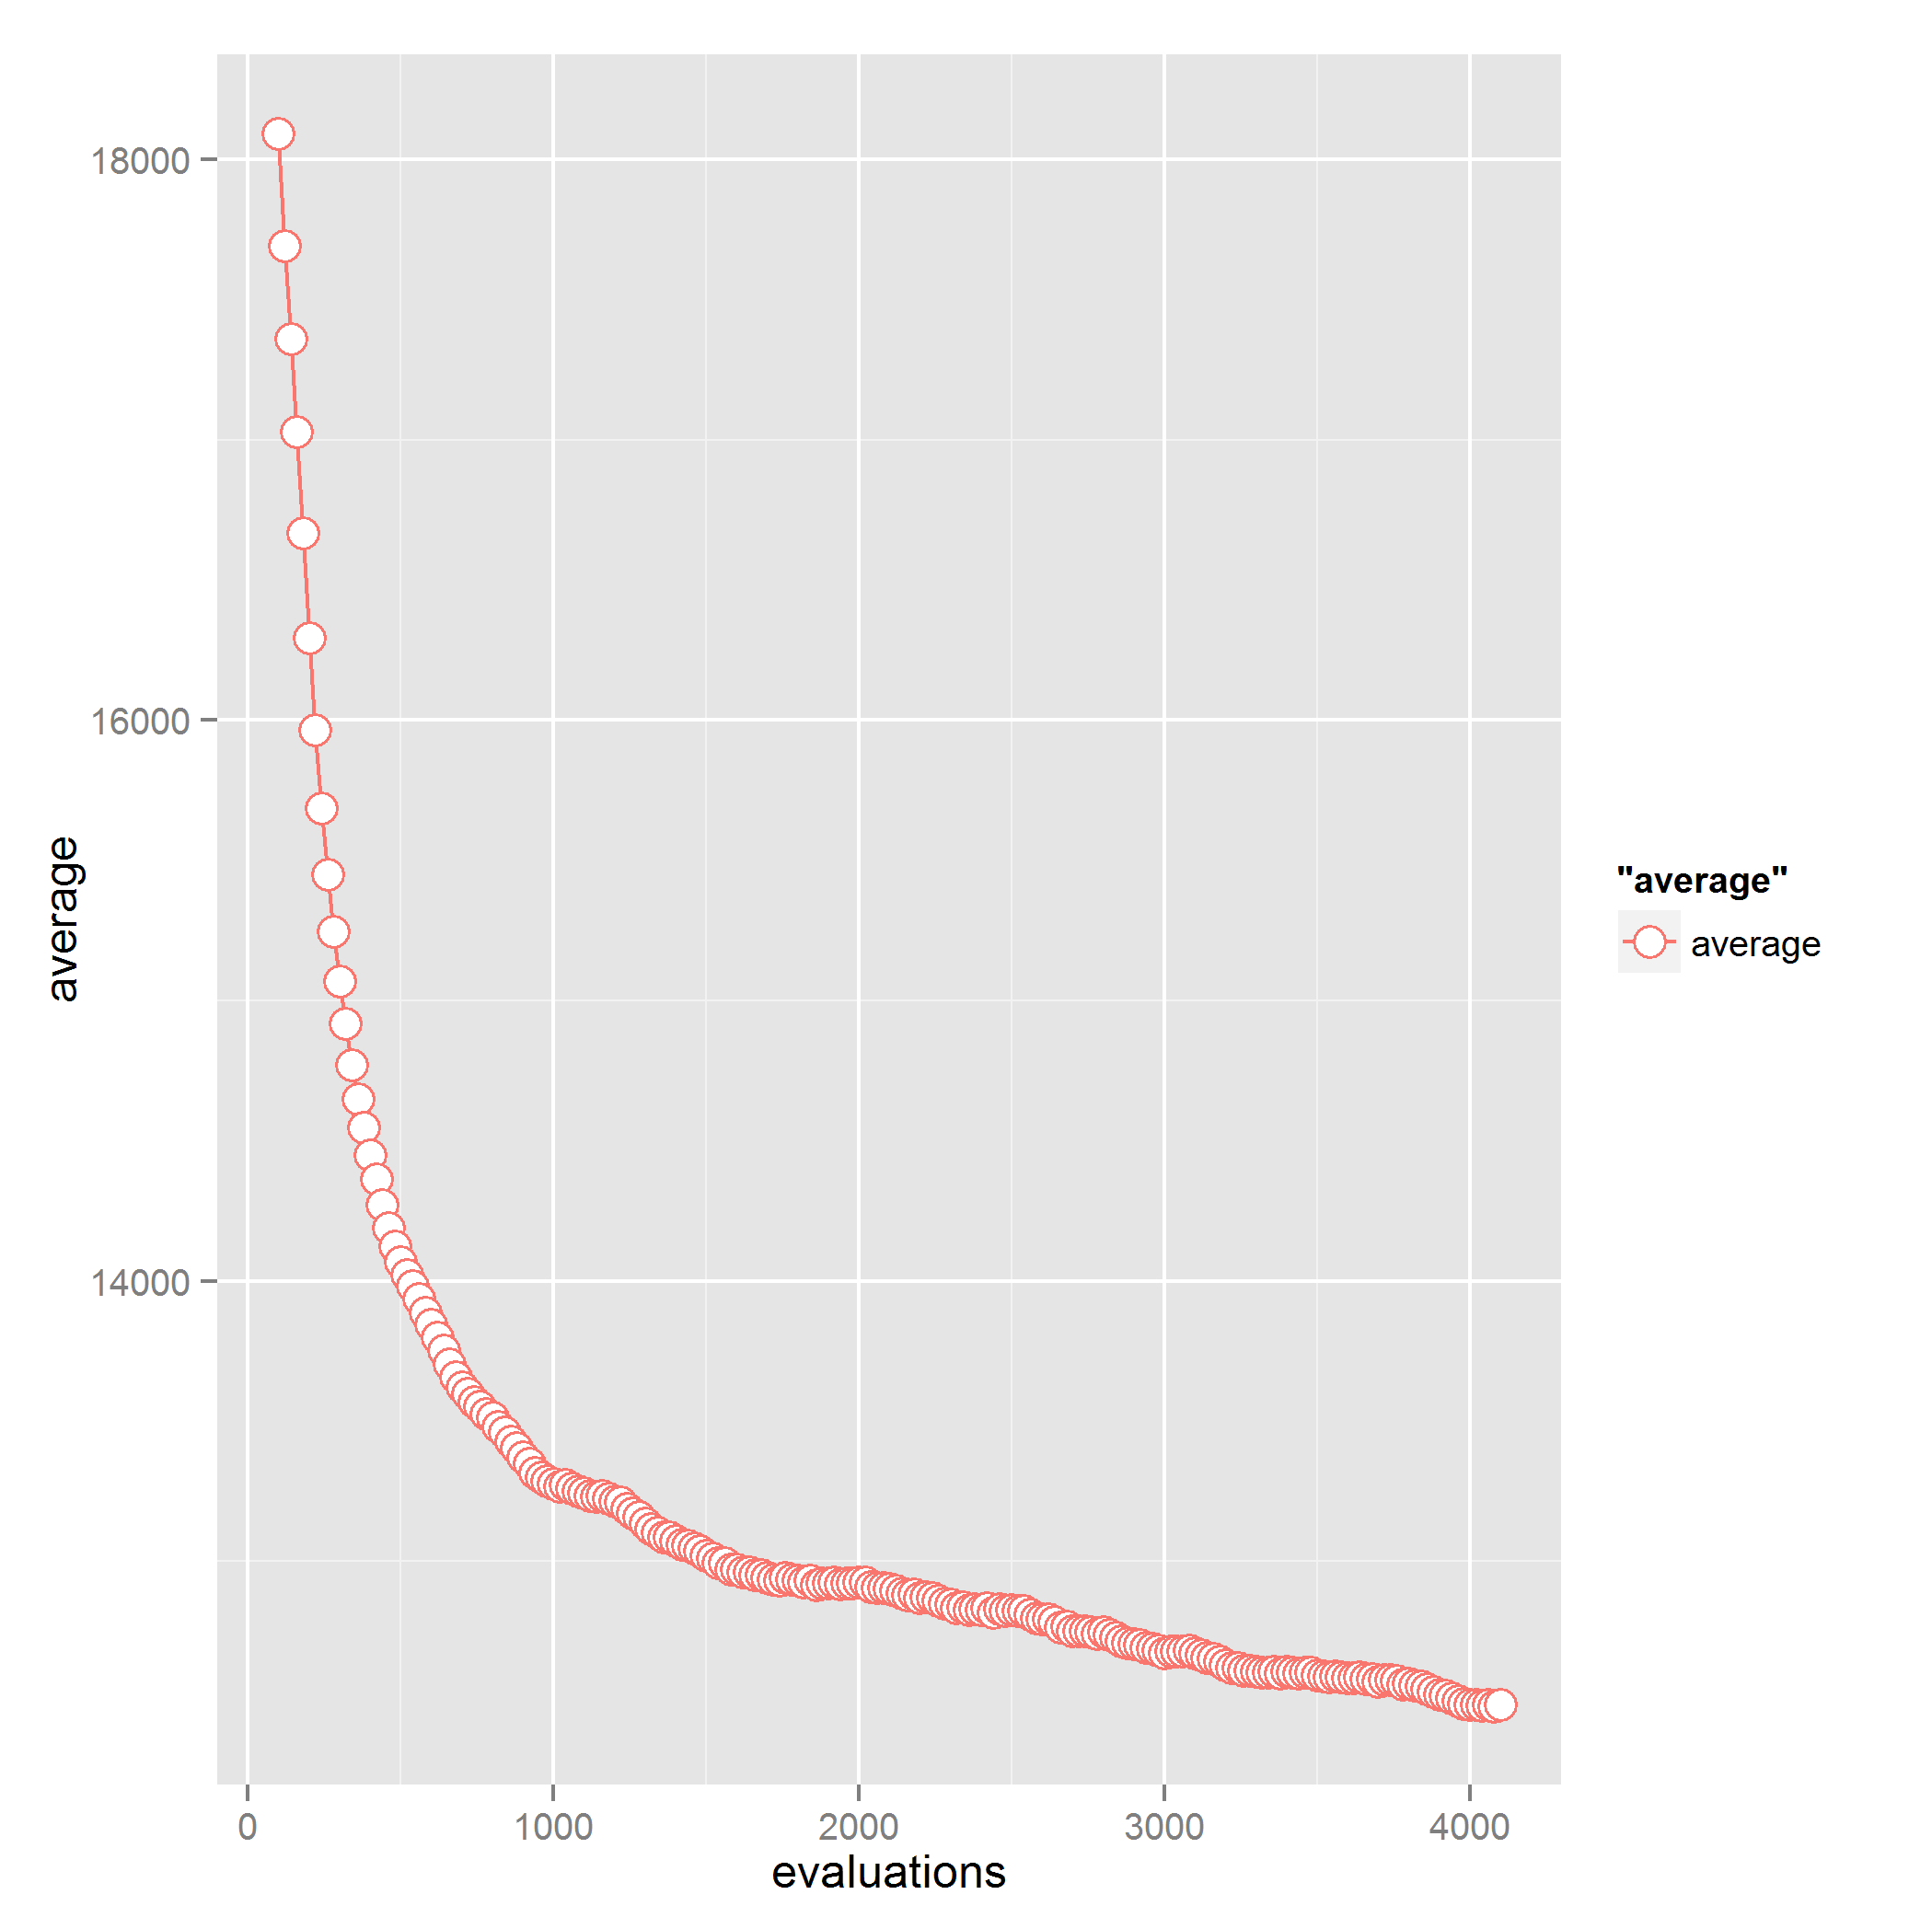
\includegraphics[]{mutation_cooling_graph2.png}

Ostatni przypadek pochodzi od hybrydy w której jako presję selekcyjną wykorzystaliśmy rozmiar turnieju. Ponieważ im większy turniej tym mniejsze prawdopodobieństwo przetrwania słabych osobników, na początku ustalilismy mały rozmiar turnieju, który stopniowo rośnie.

Mały rozmiar danych:

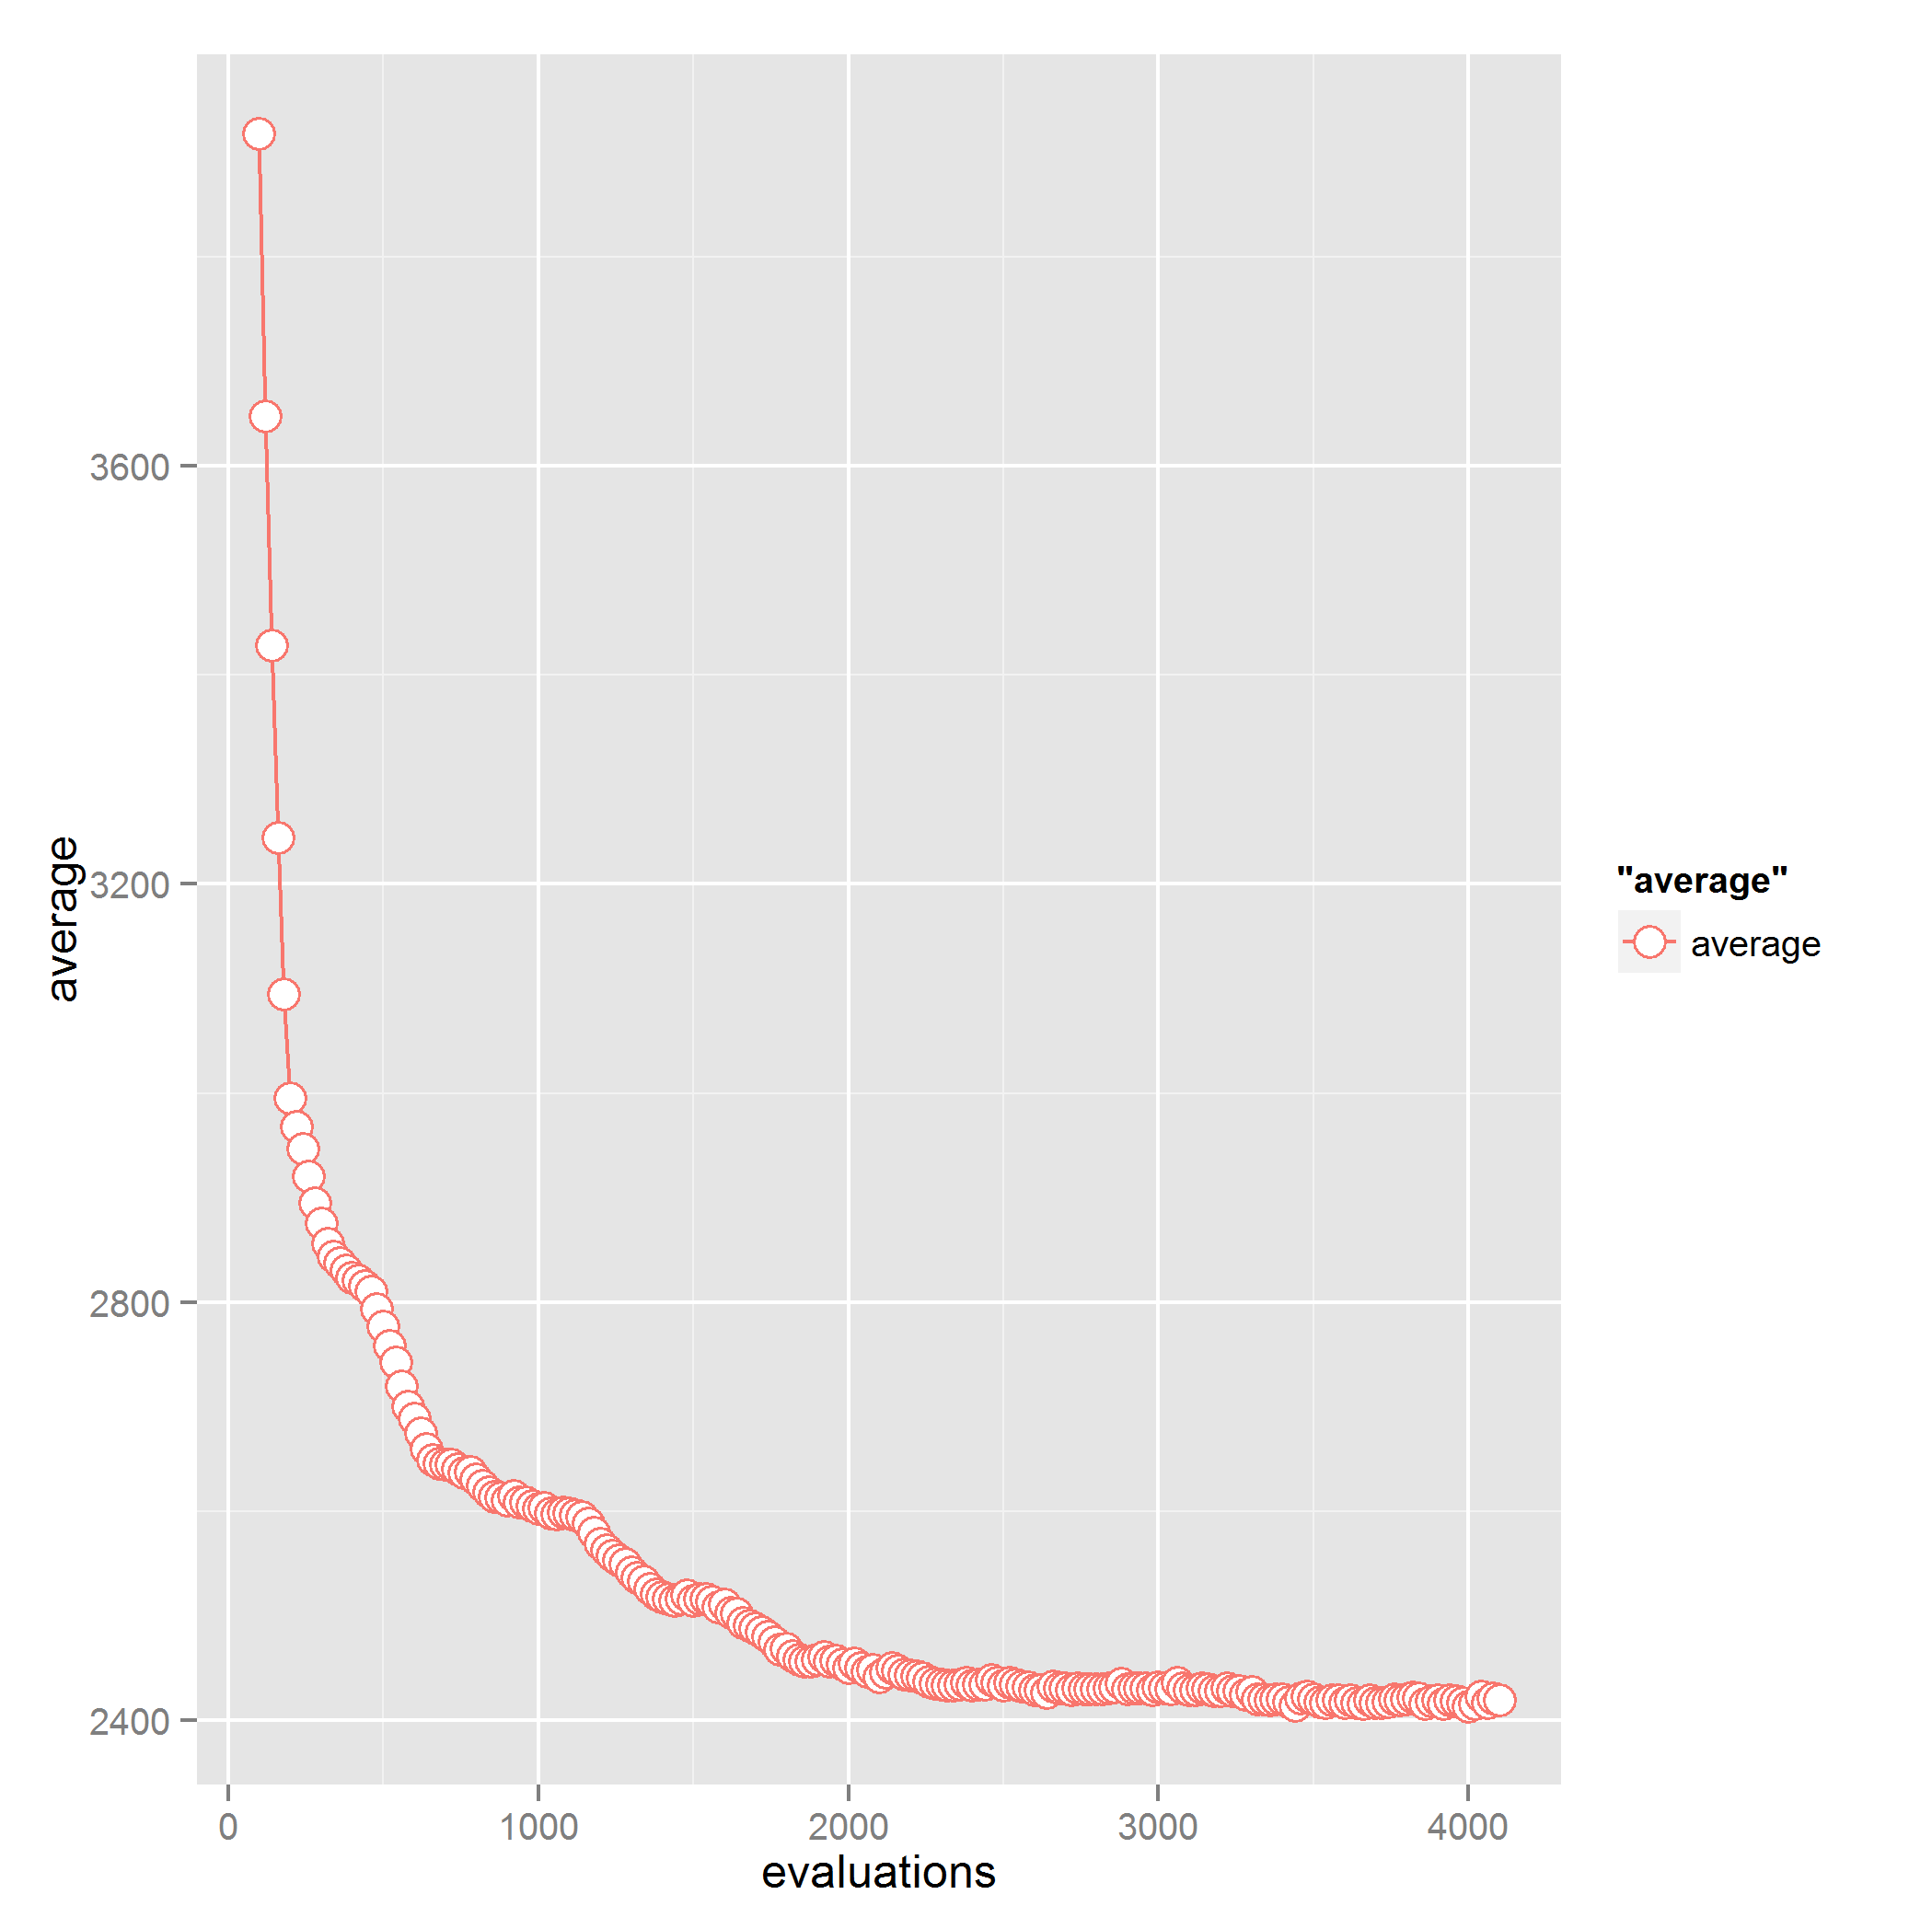
\includegraphics[]{tournament_cooling_graph0.png}

Średni rozmiar danych:

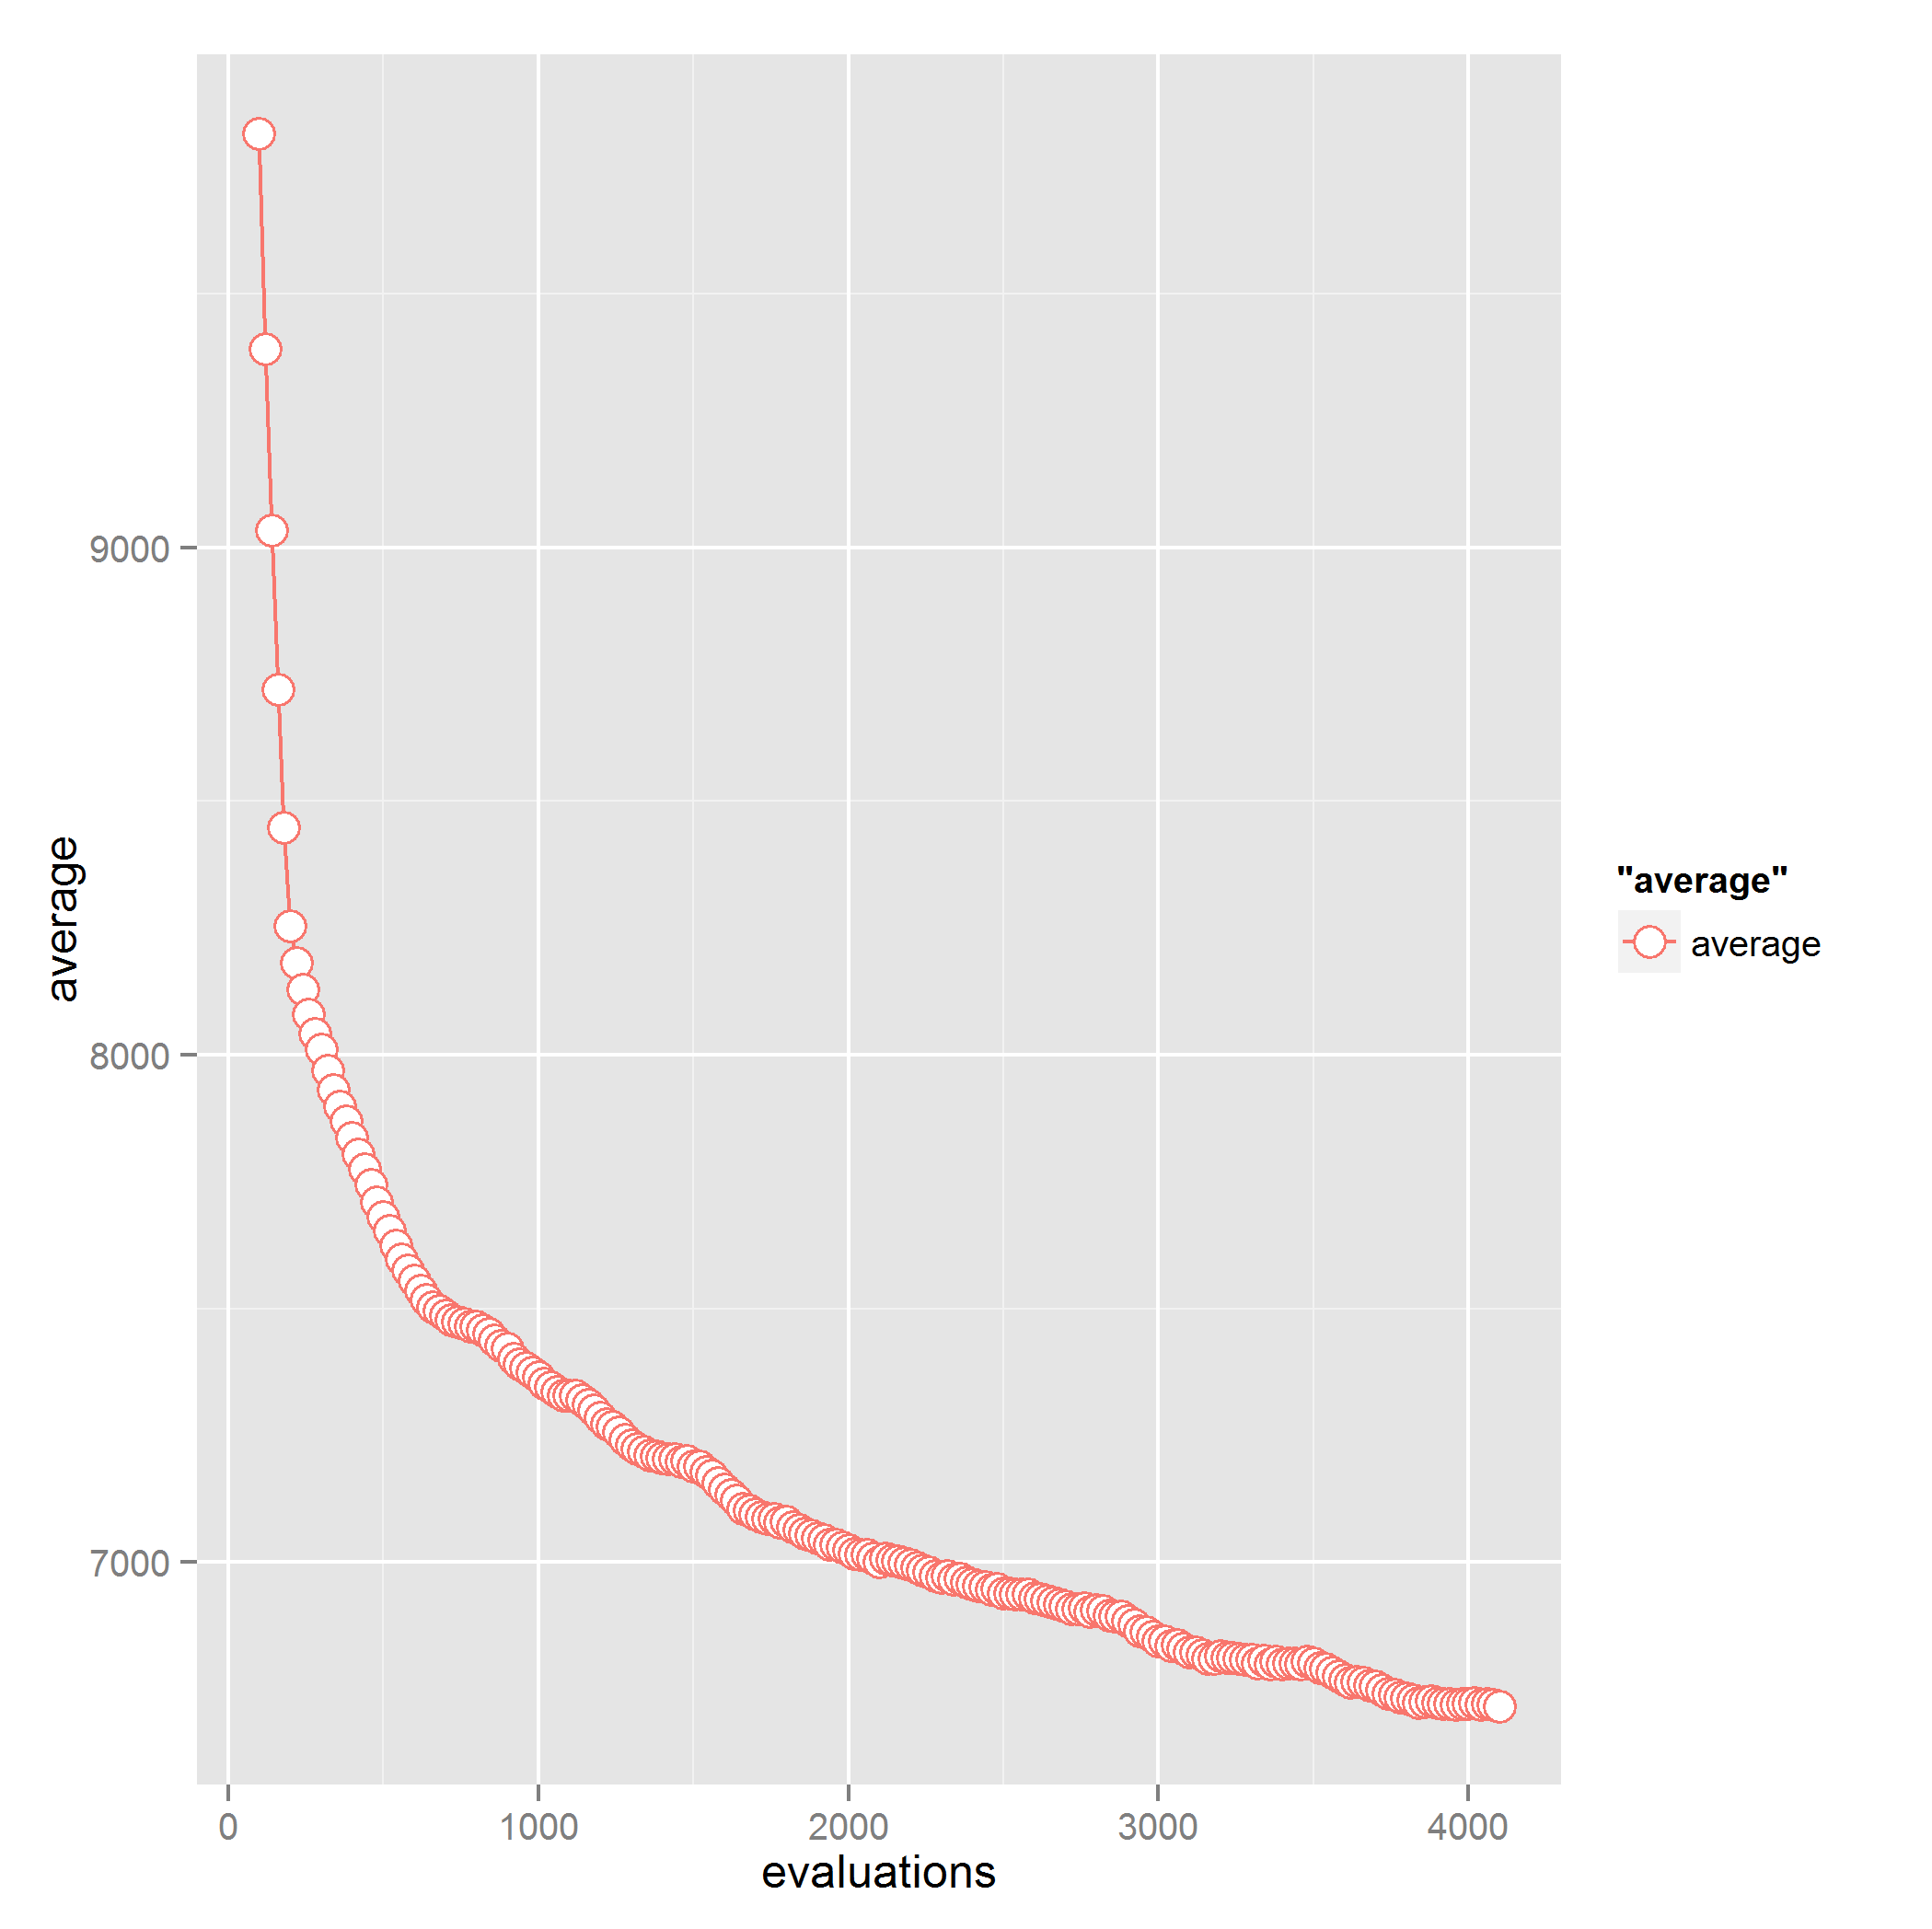
\includegraphics[]{tournament_cooling_graph1.png}

Duży rozmiar danych:

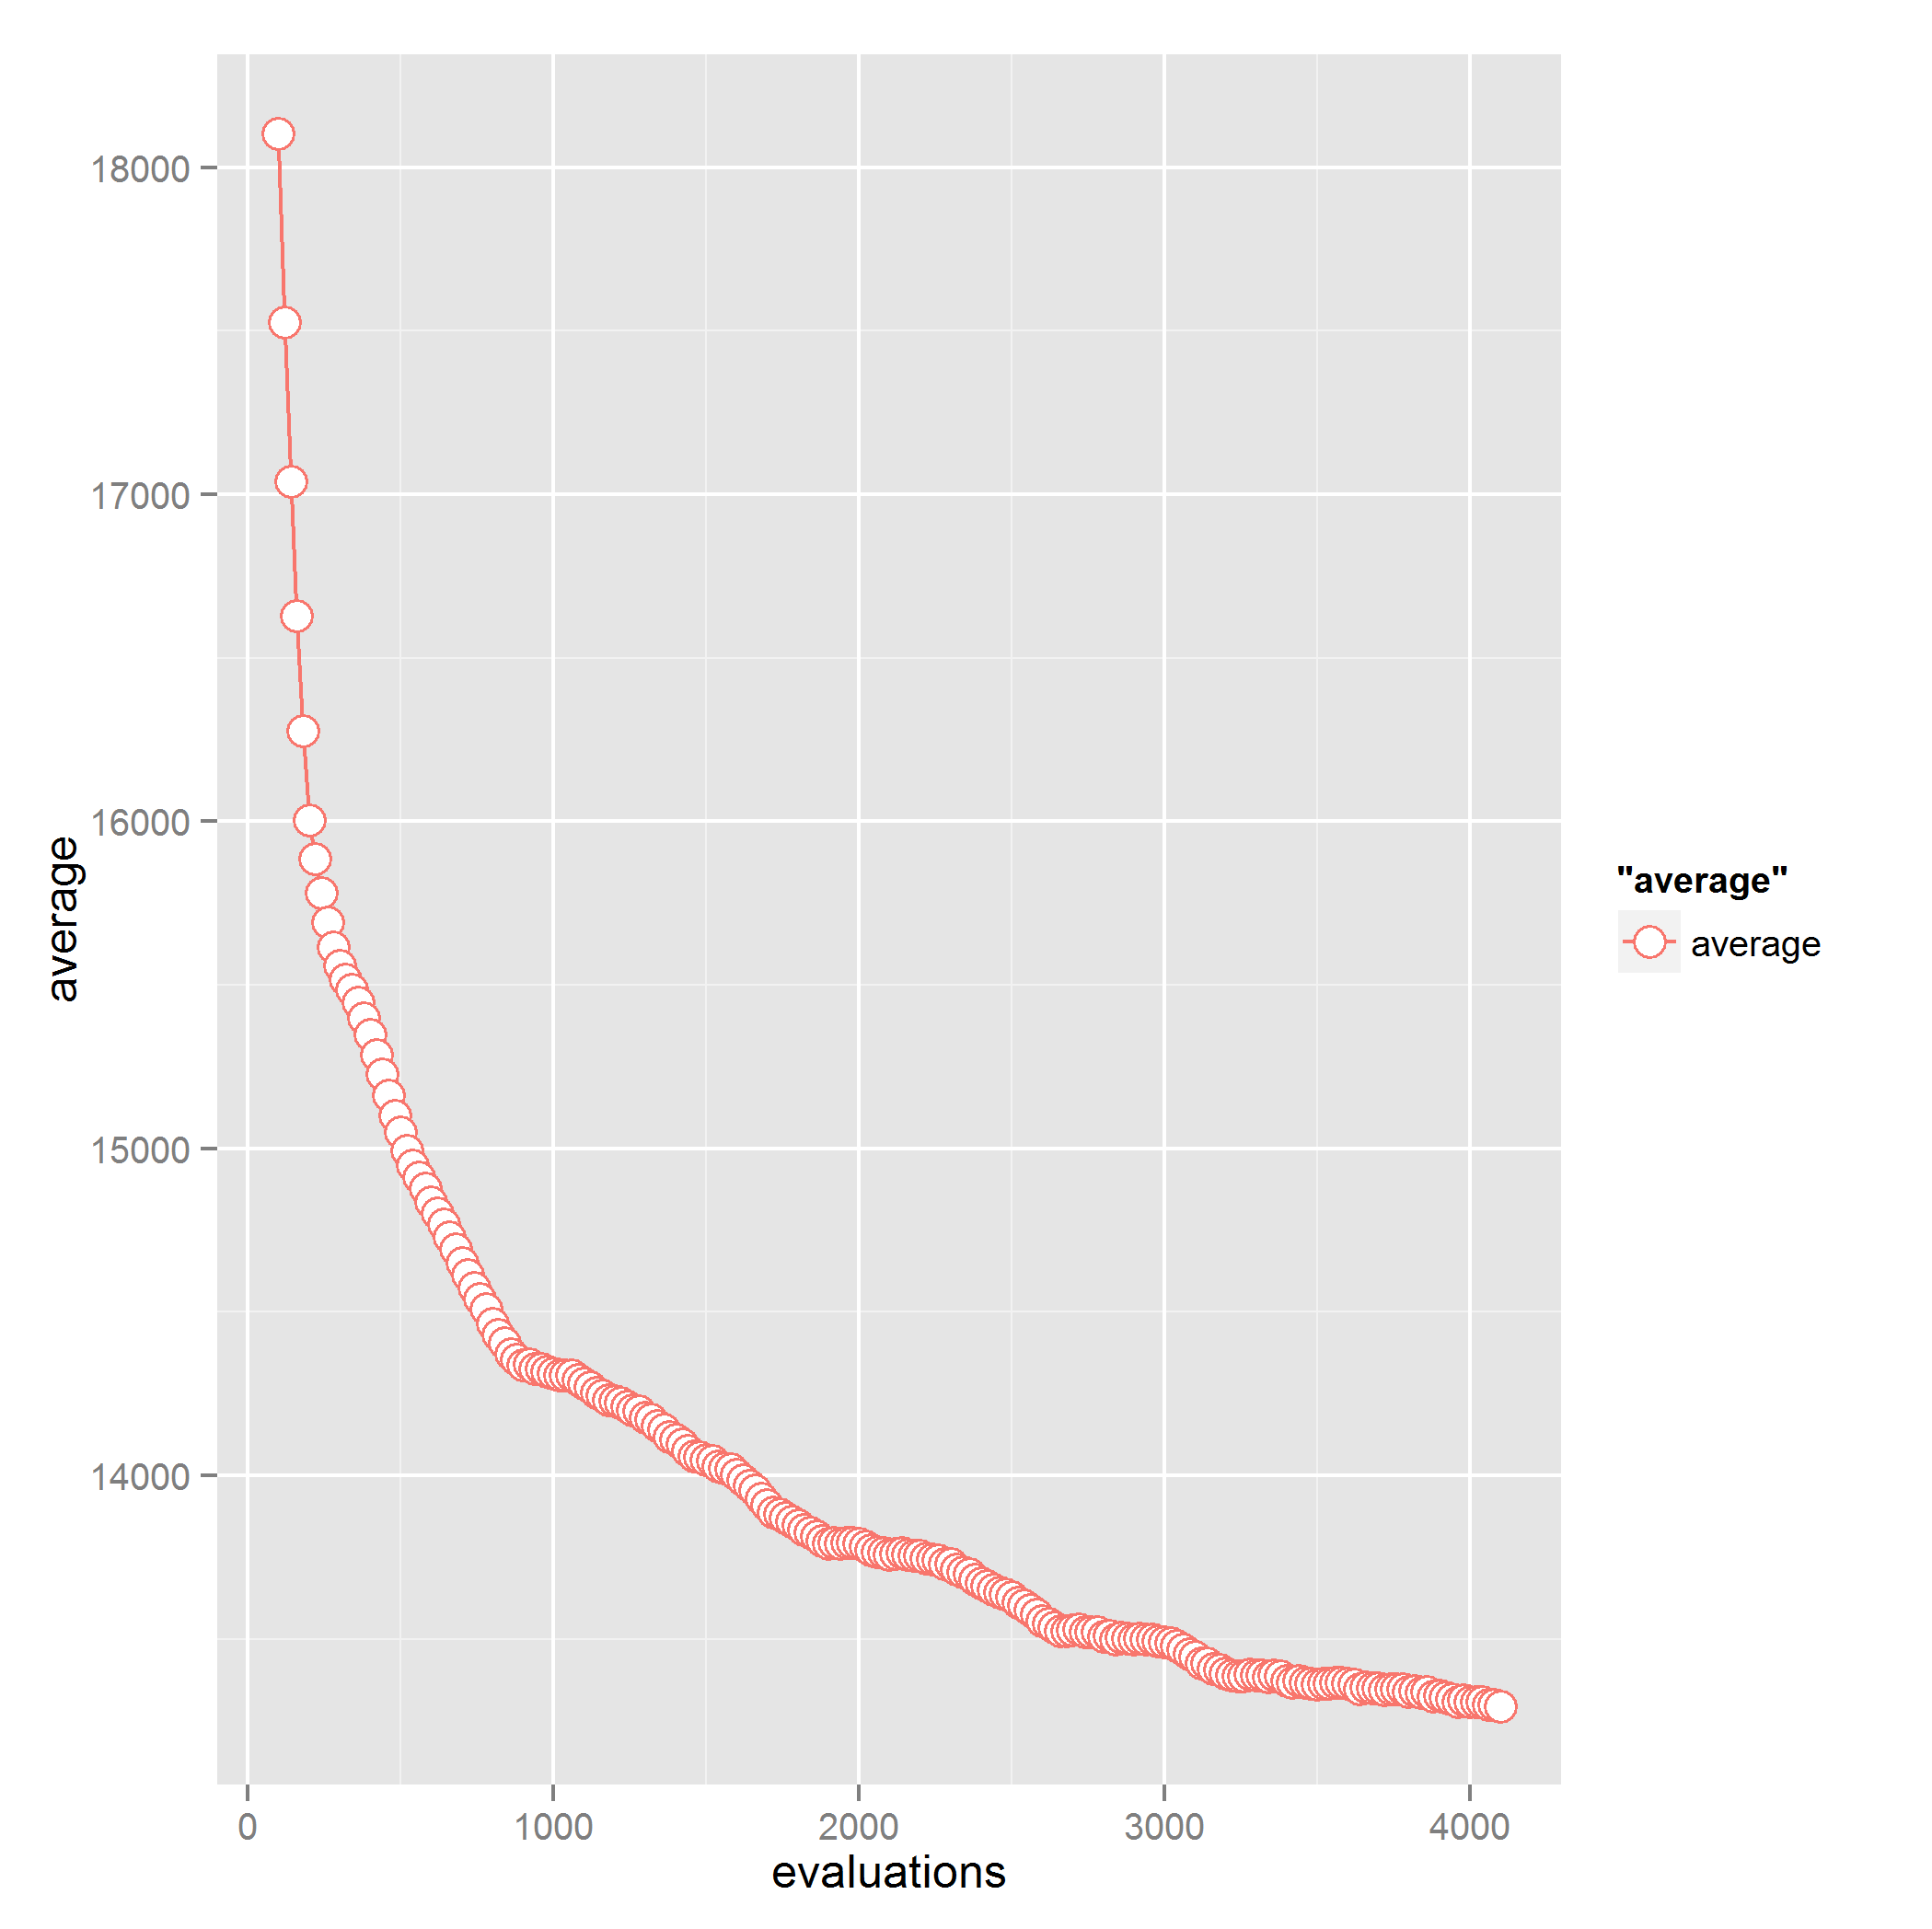
\includegraphics[]{tournament_cooling_graph2.png}

\section*{Wnioski}

Okazuje się że wbrew oczekiwaniom, najzwyklejszy algorytm genetyczny daje lepsze wyniki i jest szybciej zbieżny do optymalnego rozwiązania niż hybrydy. Obie hybrydy algorytmu genetycznego z symulowanym wyzarzaniem dają wyniki w bardzo zbliżonym czasie i są zbieżne z podobną prędkoscią. Nie jesteśmy w stanie określić jaka jest przyczyna takiego stanu rzeczy.



\bibliography{scibib}
\bibitem{Assad}
  A. Assad, W. Xu,
  \emph{The quadratic minimum spanning tree problem.}.
  Naval Research Logistics, 1992,Vol.39, 399–417.
  
\bibitem{Benchmark}
  http://homes.di.unimi.it/~cordone/research/DataQMST10-30.zip
  
  
\bibitem{Results}
  http://homes.di.unimi.it/~cordone/research/ResultsQMST.pdf

\bibliographystyle{Science}



% Following is a new environment, {scilastnote}, that's defined in the
% preamble and that allows authors to add a reference at the end of the
% list that's not signaled in the text; such references are used in
% *Science* for acknowledgments of funding, help, etc.

% For your review copy (i.e., the file you initially send in for
% evaluation), you can use the {figure} environment and the
% \includegraphics command to stream your figures into the text, placing
% all figures at the end.  For the final, revised manuscript for
% acceptance and production, however, PostScript or other graphics
% should not be streamed into your compliled file.  Instead, set
% captions as simple paragraphs (with a \noindent tag), setting them
% off from the rest of the text with a \clearpage as shown  below, and
% submit figures as separate files according to the Art Department's
% instructions.


\clearpage

\end{document}




















